\documentclass[11pt]{My_preprint}

\title{
    Buoyancy driven motion of non-coalescing inertial drops: 
    analysis and modeling of the microstructure kinematic with nearest particle statistics. 
}

\author[1,2]{Nicolas Fintzi}
\author[1]{Jean-Lou Pierson}
\author[2]{Stephane Popinet}
\affil[1]{IFP Energies Nouvelles, Rond-point de l’echangeur de Solaize, 69360 Solaize}
\affil[2]{Sorbonne Universit\'e, Institut Jean le Rond d'Alembert, 4 place Jussieu, 75252 PARIS CEDEX 05, France}
\normalmarginpar


\begin{document}

\maketitle

\begin{abstract}
    In this study, we provide a comprehensive analysis of the various  arrangements that droplets can adopt within dispersed buoyant emulsions. 
    This is termed the study of the microstructure.
    To this end, we have developed a novel algorithm capable of effectively prevents numerical coalesce between drops at reasonable computational cost.
    This algorithm is implemented within the Volume of Fluid (VoF) method, utilizing the \href{http://basilisk.fr}{http://basilisk.fr} open source code. 
    Subsequently, we conducted Direct Numerical Simulations (DNS) of statistically steady state mono-disperse buoyant emulsion, over a broad range of \textit{Galileo} number ($Ga$), particle volume fraction ($\phi$), and viscosity ratio ($\lambda$). 
    The density ratio and the \textit{Bond} number are kept constant, $\zeta = 1.11$ and  $Bo = 0.2$, respectively. 
    Then it is shown that, as predicted by \citet{zhang2023evolution}, the second moment of the nearest particle pair distribution, noted \textbf{R}, has the capability to quantify microstructure's features such as clusters and layers of particles.
    In particular, it is found that : 
    (1) At low $Ga$ isotropic clusters appear with increasing $\phi$. 
    (2) Non-isotropic clusters such as layers of particles, are more likely to form for high \textit{Galileo} number.
    (3) The viscosity ratio $\lambda$ has an important impact on the microstructure, clearly more layers are formed for $\lambda = 1$ than $\lambda = 10$. 
    Overall, our study provides a quantitative measure of the microstructure geometry 
     in terms of $Ga$, $\phi$ and $\lambda$. 
\end{abstract}

\section{Introduction}





\begin{enumerate}
    \item We use extensively averaged models in industry 
    \item These models necessitate closure laws. These closure laws are highly dependent on the particles' microstructure. 
    \item In our previous work we performed a \textit{Nearest-particle-statistics} analysis of the microstructure geometry, or the steady state microstructure. 
    \item All the closures in the literature are performed in steady state system. 
    Therefore, in order to be valid in a Euler-Euler averaged context the time scales of the simulation must be greater than the time for the microstructure to reach its steady state. 
    Only then the assumption of quasi steady ness is valid.    
    \item Therefore, in this study we provide a theoritical and numerical analyssi of the timescale that drives the microstructure. 
    Doing so, we demonstrate that the particle interaction time is the main timescale involved in the microstructure relaxation time. 
    We therefor also study the relative kinematic
\end{enumerate}

% \subsection{Numerical method}

In this problem, the governing equations consist of the one-fluid formulation of the mass and momentum equation, with an additional transport equation for the dispersed phase indicator function. 
We recall their form here, 
\begin{align}
    \pddt \rho+ \div(\rho\textbf{u})
    &= 0,\\
    \label{eq:dt_urho}
    \pddt (\rho \textbf{u})
    + \div (\rho  \textbf{u} \textbf{u} - \bm\sigma)
    &= (\avg{\rho} - \rho)\textbf{g}
    + \textbf{f}_\gamma,\\
    \label{eq:dt_C}
    \pddt C + \textbf{u}\cdot\grad C  
    &= 0,
\end{align}
% \tb{mettre le link navier stokes solver et faire ca pour le reste }
which are the mass, momentum and colors function transport equation, respectively. 
The scalar fields $C$, represents the color function, which range between $0$ and $1$ to indicate the proportion of fluid and dispersed phase, respectively. 
We introduced the fluid velocity vector $\textbf{u}$ and the Newtonian stress tensor $\bm{\sigma} = -p \textbf{I} + \mu (\grad \textbf{u}+ \grad \textbf{u}^\dagger)$ where $p$ is the pressure fields and $^\dagger$ represents the transpose operator.
Note that the material properties, $\rho$ and $\mu$, take the value of the phases in presence, following the arithmetic average : $\rho = (1-C)\rho_f + C \rho_d$ and $\mu = (1-C)\mu_f + C \mu_d$. 
In our case the arithmetic mean turns out to perform better compared to the harmonic mean, which is often used to interpolate the viscosity for bubbly flows \citet{hidman2023assessing,innocenti2020direct}.
More details about this choice is provided in \ref{ap:validation} (\textit{Case 1.}). 
The capillary force is defined as, $\textbf{f}_\gamma =\textbf{n} \gamma \div \textbf{n} $, where \textbf{n} is the normal at the interface.
Following  \citep{bunner2002dynamics}, we incorporated the artificial body force term, $\avg{\rho}\textbf{g}$, on the right-hand side of \ref{eq:dt_urho}, to maintain a zero-averaged velocity throughout the entire numerical domain.  

To solve these equations we first initialized $125$ spherical droplets within a cubic domain with fully periodic boundary condition. 
We used the open source code \url{http///basilisk.fr} to discretize the governing equations in a multigrid solver. 
The Navier-Stokes equations are discretized with a centered scheme.
The two-phase flow solver uses the Volume of Fluid (VoF) method. 
The interfaces between the droplets and the carrier fluid is reconstructed using the Piecewise Linear Inter-face Calculation or PLIC method \citet[Chapter 5.]{tryggvason2011direct}.
Regarding the treatment of the surface tension force term we refer the reader to \citet{popinet2018numerical} for more details. 
The Basilisk solver has been validated extensively, in the framework of bubbly flow. 
Most of the previous studies \citep{hidman2023assessing,innocenti2020direct} recommend a grid definition of $\Delta/d \ge  30$, where $\Delta$ is the grid spacing. 
In \ref{ap:validation} we carried a mesh independence study and demonstrate that a grid spacing of $\Delta = d/30$ is also suitable in our context.
For readers seeking more detailed information about the solvers, we recommend the wiki pages : \href{http://basilisk.fr/src/navier-stokes/centered.h}{centered.h}, \href{http://basilisk.fr/src/tension.h}{tension.h} and \href{http://basilisk.fr/src/poissson.h}{poissson.h} where he can find the source code of the Navier-Stokes, surface tension and multigrid solver used in this work, respectively. 

With the VoF method droplets and bubbles may experience premature coalesce.
For a detailed discussion on this issue, see  \citet[Appendix B]{innocenti2020direct}.
However, in this work, it is imperative to conserve a specific (mono-disperse) population of droplets over time to accumulate sufficient statistics about the microstructure.
To tackle this issue we present in the next section a novel algorithm which prevent coalescence between droplets, while maintaining a reasonable cost. 







\section{Theoretical framework}
\label{sec:Theory}

In the continuity of \citet{fintzi2024buoyancy} we study the microstructure of emulsion using the \textit{Nearest-Particle Statistics} (NPS) framework. 
Particularly, we will be interested in the age-included nearest-pair probability density function \citep{zhang2021ensemble}. 
In addition to give details about relative positions this probability density provides information regarding the time of interaction between the nearest particle pairs. 

\subsection{The age-included nearest-pair probability density function}
Let $P(\FF)$ be the probability density function that describes the probability of finding the flow in the configuration $\FF$.
Then, we define $d\mathscr{P} = P(\FF)d\FF$ as the probable number of realizations in the incremental region of the flow' phase space, $d\FF$ around $\FF$.
The vectors  $\textbf{x}_i(t,\FF)$ and $\textbf{x}_j(\FF,t)$ refer to the position of the particles $i$ and $j$ at time $t$ for a configuration $\FF$, respectively. 
Additionally, the time $t_{ij}(\FF)$, is the time at which the particles $i$ and $j$ became nearest neighbor.
This Lagrangian quantity is a constant scalar fixed in time and may change according to the flow configuration $\FF$.
Based on these Lagrangian quantities we can define The age-included nearest pair distribution function as \citep{zhang2023evolution},
\begin{equation}
    P_{nst}(\textbf{x},\textbf{r},a,t) =
    \int \sum_{i}^{N_b}\delta[\textbf{x}-\textbf{x}_i(t,\FF)]
    \sum_{j\neq i}^{N_b}\delta[\textbf{x}+\textbf{r}-\textbf{x}_j(t,\FF)]
    \delta[t+a-t_c^{ij}(\FF)] 
    h_{ij} (t,\FF)
    d\mathscr{P},
    \label{eq:P_nstij}
\end{equation}
where
\begin{equation*}
    h_{ij}(\FF,t)
    = \left\{
        \begin{tabular}{cc}
            $1/N_i(\FF,t)$ & if $j$ is one of the $N^{th}$ nearest neighbors of $i$ \\
            0& otherwise
        \end{tabular}
        \right.,
\end{equation*}
Here $\textbf{x}$ and $\textbf{r}$ are coordinate vectors in $\mathbb{R}^3$ and $a \geq 0 $ is the \textit{age} of interaction, i.e. the current time minus the time at which both particle became nearest neighbors.   
With this definition $P_{nst}(\textbf{x},\textbf{r},t,a)$ is the probability of finding a particle at \textbf{x} and time $t$, with a nearest neighbor at the position $\textbf{x}+\textbf{r}$ with age $a$.
We also introduce the \textit{reduced} nearest neighbor distributions, they read as
\begin{align}
    P_\text{r}(\textbf{r}|\textbf{x},t)
    =\frac{1}{n_p(\textbf{x},t)}\int_0^\infty P_\text{nst}(\textbf{x},\textbf{r},t,a) da,\\
    P_a(a|\textbf{x},t)
    = \frac{1}{n_p(\textbf{x},t)}\int_{\mathbb{R}^3} P_\text{nst}(\textbf{x},\textbf{r},t,a) d\textbf{r},
\end{align}
where $P_r(\textbf{r}|\textbf{x},t)$ represents the probability of finding a nearest neighbor at $\textbf{x}+\textbf{r}$ knowing that a particle is already present at \textbf{x} and time $t$, regardless of the age of interaction. 
And $P_a(a|\textbf{x},t)$ is the probability of finding  a nearest-neighboring particles having age $a$, regardless of the relative position, knowing a particle is present at \textbf{x} and time $t$. 
Note that these distribution functions are all normalized such that 
\begin{equation}
    \frac{1}{n_p(\textbf{x},t)}\int_0^\infty \int_{\mathbb{R}^3} P_\text{nst}(\textbf{x},\textbf{r},t,a) d\textbf{r} da 
    = 
    \int_{\mathbb{R}^3} P_\text{r}(\textbf{x},\textbf{r},t) d\textbf{r} 
    = \int_0^\infty P_\text{a}(\textbf{x},\textbf{r},t) da 
    = 1,
    \label{eq:eq_n_p}
\end{equation}
with $n_p(\textbf{x},t)$ the number density function, defined as
\begin{equation}
    n_p(\textbf{x},t)= 
    \int \sum_{i}^{N_b}\delta[\textbf{x}-\textbf{x}_i(t,\FF)] d\mathscr{P}.
    \label{eq:n_p}
\end{equation}


In addition to these distribution functions we also wish to analyze the relative kinematic between nearest neighbors. 
To that end we introduce the Lagrangian relative velocity $\textbf{w}_{ij}(t,\FF) = \textbf{u}_j(t,\FF) - \textbf{u}_i(t,\FF)$, with $\textbf{u}_i(t,\FF)$ and $\textbf{u}_j(t,\FF)$, the center of mass velocity of the particle $i$ and $j$, respectively.
The conditional average of the Lagrangian relative velocity can be written
\begin{equation*}
    \textbf{w}^\text{nst}_p (\textbf{x},\textbf{r},t,a)
    = 
    \frac{1}{P_{nst}(\textbf{x},\textbf{r},t,a)}
    \int \sum_{i}^{N_b}\delta(\textbf{x}-\textbf{x}_i)
    \sum_{j\neq i}^{N_b}\delta(\textbf{x}+\textbf{r}-\textbf{x}_j) 
    \delta(t+a-t_c^{ij}) 
    \textbf{w}_{ij}
    h_{ij} 
    d\mathscr{P}.
    \label{eq:q_nstij}
\end{equation*}
Following this definition, $\textbf{w}^\text{nst}_p(\textbf{x},\textbf{r},t,a)$ is the averaged relative velocity between two nearest neighboring particles, one of which is situated at $\textbf{x}$ and time $t$, with its nearest neighbor at $\textbf{x}+\textbf{r}$ with age $a$. 
The physical meaning of such a field will be further investigated in \ref{sec:velocity}. 
For instance, note that the subscript $_p$ indicates that $\textbf{w}^\text{nst}_p$ is at the origin a Lagrangian property, it is therefore averaged conditionally on the presence of a particle at $\textbf{x}$ and time $t$. 
Whereas superscript $^\text{nst}$ indicates that $\textbf{w}_{ij}(\FF,t)$ is conditionally averaged on the presence of a nearest neighbor at $\textbf{x}+\textbf{r}$ with age $a$. 

In general, $\textbf{w}_{ij}(t,\FF)$ can be replaced by any particle's properties. 
An example particularly interesting in this work is the particle absolute velocity $\textbf{u}_i(\FF,t)$.
In this case, $\textbf{u}^\text{nst}_p(\textbf{x},\textbf{r},t,a)$ represents the averaged velocity of the particles, given that a particle is present at \textbf{x} and time $t$, with its nearest neighbor located at $\textbf{x}+\textbf{r}$ with age $a$. 
Using the property of the nearest neighbor distribution functions we deduce that  $\textbf{u}^\text{nst}_p$ is related to the ensemble averaged particle phase velocity, defined as 
\begin{equation*}
    \textbf{u}_p(\textbf{x},t)=\frac{1}{n_p(\textbf{x},t)} 
    \int \sum_{i}^{N_b}\delta[\textbf{x}-\textbf{x}_i(t,\FF)]  \textbf{u}_i(t,\FF)d\mathscr{P},
\end{equation*}
through the relation
\begin{equation}
    \textbf{u}_p = \frac{1}{n_p(\textbf{x},t)} \int_0^\infty \int_{\mathbb{R}^3} \textbf{w}_p^\text{nst} P_\text{nst}(\textbf{x},\textbf{r},t,a) d\textbf{r} da. 
    \label{eq:u_p}
\end{equation}



\subsection{A transport equation to describe the evolution of the microstructure}

In our previous work \citep{fintzi2024buoyancy} we have seen that the tensor,
\begin{equation}
    \textbf{R}(\textbf{x},t)
    = \frac{1}{n_p(\textbf{x},t)}
    \int_0^\infty 
    \int_{\mathbb{R}^3}
    \textbf{rr}
    P_\text{nst}(\textbf{x},\textbf{r},a,t)
    d\textbf{r}
    da
    \label{eq:R}
\end{equation}
is able to describe the particles arrangements, or microstructure.
Specifically, it was shown that $\textbf{R}(\textbf{x},t)$ measures features such as layers or clusters of particles. 
The scalar $R = \bm\delta:\textbf{R}(\textbf{x},t)$ with $\bm\delta$ the unit tensor, represents the averaged mean square distance to the nearest neighbors.
And the deviatoric part of this tensor, namely $\textbf{A} = \textbf{R}-\frac{1}{3}R\bm\delta$, measures the anisotropy of the microstructure. 
\ref{fig:scheme_clusters} provides a concise explanation of the implications of the values of $\textbf{A}$ and $R$ on the microstructure.  
\begin{figure}[h!]
    \hfill
\begin{tikzpicture}
    \draw[<->] (-1.5,1)node[right]{$y$}--++(0,-1)--++(1,0)node[right]{$x$};
    % \draw[->] (-1,2.5)--++(0,-2)node[midway, left]{$\textbf{g}$};
    \foreach \i in {1,...,5} {
    \pgfmathsetmacro{\x}{rnd}
    \pgfmathsetmacro{\y}{rnd}
    \draw[fill=gray!50] ($(\x,\y)$) circle (0.1);
    }
    \foreach \i in {1,...,5} {
    \pgfmathsetmacro{\x}{rnd}
    \pgfmathsetmacro{\y}{rnd}
    \draw[fill=gray!50] ($(\x+1,\y)$) circle (0.1);
    }
    \foreach \i in {1,...,5} {
    \pgfmathsetmacro{\x}{rnd}
    \pgfmathsetmacro{\y}{rnd}
    \draw[fill=gray!50] ($(\x+2,\y)$) circle (0.1);
    }
    \foreach \i in {1,...,5} {
        \pgfmathsetmacro{\x}{rnd}
        \pgfmathsetmacro{\y}{rnd}
        \draw[fill=gray!50] ($(\x+1,\y+1)$) circle (0.1);
    }
    \foreach \i in {1,...,5} {
    \pgfmathsetmacro{\x}{rnd}
    \pgfmathsetmacro{\y}{rnd}
    \draw[fill=gray!50] ($(\x+2,\y+1)$) circle (0.1);
    }
    \foreach \i in {1,...,5} {
    \pgfmathsetmacro{\x}{rnd}
    \pgfmathsetmacro{\y}{rnd}
    \draw[fill=gray!50] ($(\x,\y+1)$) circle (0.1);
    }
    \foreach \i in {1,...,5} {
        \pgfmathsetmacro{\x}{rnd}
        \pgfmathsetmacro{\y}{rnd}
        \draw[fill=gray!50] ($(\x+1,\y+2)$) circle (0.1);
    }
    \foreach \i in {1,...,5} {
    \pgfmathsetmacro{\x}{rnd}
    \pgfmathsetmacro{\y}{rnd}
    \draw[fill=gray!50] ($(\x+2,\y+2)$) circle (0.1);
    }
    \foreach \i in {1,...,5} {
    \pgfmathsetmacro{\x}{rnd}
    \pgfmathsetmacro{\y}{rnd}
    \draw[fill=gray!50] ($(\x,\y+2)$) circle (0.1);
    }
    \draw (1.5,3.4)node[below]{\textit{Case 1}};
    \draw (1.5,0)node[below]{$\textbf{A}\approx \bm 0$ \& $R\approx r_m^2$};
\end{tikzpicture}
\hfill
\begin{tikzpicture}
    \foreach \i in {1,...,5} {
    \pgfmathsetmacro{\x}{rnd*0.4}
    \pgfmathsetmacro{\y}{rnd*0.4}
    \draw[fill=gray!50] ($(\x,\y)$) circle (0.1);
    }
    \foreach \i in {1,...,5} {
    \pgfmathsetmacro{\x}{rnd*0.3}
    \pgfmathsetmacro{\y}{rnd*0.3}
    \draw[fill=gray!50] ($(\x+1,\y)$) circle (0.1);
    }
    \foreach \i in {1,...,5} {
    \pgfmathsetmacro{\x}{rnd*0.3}
    \pgfmathsetmacro{\y}{rnd*0.3}
    \draw[fill=gray!50] ($(\x+2,\y)$) circle (0.1);
    }
    \foreach \i in {1,...,5} {
        \pgfmathsetmacro{\x}{rnd*0.5}
        \pgfmathsetmacro{\y}{rnd*0.5}
        \draw[fill=gray!50] ($(\x+0.5,\y+1)$) circle (0.1);
    }
    \foreach \i in {1,...,5} {
        \pgfmathsetmacro{\x}{rnd*0.4}
        \pgfmathsetmacro{\y}{rnd*0.4}
        \draw[fill=gray!50] ($(\x+2.5,\y+1)$) circle (0.1);
    }
    \foreach \i in {1,...,5} {
        \pgfmathsetmacro{\x}{rnd*0.4}
        \pgfmathsetmacro{\y}{rnd*0.4}
        \draw[fill=gray!50] ($(\x+1.5,\y+1)$) circle (0.1);
        }
    \foreach \i in {1,...,5} {
        \pgfmathsetmacro{\x}{rnd*0.5}
        \pgfmathsetmacro{\y}{rnd*0.5}
        \draw[fill=gray!50] ($(\x,\y+2)$) circle (0.1);
    }
    \foreach \i in {1,...,5} {
        \pgfmathsetmacro{\x}{rnd*0.4}
        \pgfmathsetmacro{\y}{rnd*0.4}
        \draw[fill=gray!50] ($(\x+2,\y+2)$) circle (0.1);
    }
    \foreach \i in {1,...,5} {
        \pgfmathsetmacro{\x}{rnd*0.4}
        \pgfmathsetmacro{\y}{rnd*0.4}
        \draw[fill=gray!50] ($(\x+1,\y+2)$) circle (0.1);
        }
    \draw (1.5,3.4)node[below]{\textit{Case 2}};
    \draw (1.5,0)node[below]{$\textbf{A}\approx \bm 0$ \& $R < r_m^2$};
\end{tikzpicture}
\hfill
\begin{tikzpicture}
    \foreach \i in {1,...,5} {
    \pgfmathsetmacro{\x}{rnd*1.5}
    \pgfmathsetmacro{\y}{rnd*0.2}
    \draw[fill=gray!50] ($(\x,\y)$) circle (0.1);
    }
    \foreach \i in {1,...,5} {
    \pgfmathsetmacro{\x}{rnd*1.5}
    \pgfmathsetmacro{\y}{rnd*0.3}
    \draw[fill=gray!50] ($(\x+1,\y)$) circle (0.1);
    }
    \foreach \i in {1,...,5} {
    \pgfmathsetmacro{\x}{rnd*1.5}
    \pgfmathsetmacro{\y}{rnd*0.3}
    \draw[fill=gray!50] ($(\x+2,\y)$) circle (0.1);
    }
    \foreach \i in {1,...,5} {
        \pgfmathsetmacro{\x}{rnd*1.5}
        \pgfmathsetmacro{\y}{rnd*0.2}
        \draw[fill=gray!50] ($(\x+1+0.5,\y+1)$) circle (0.1);
    }
    \foreach \i in {1,...,5} {
    \pgfmathsetmacro{\x}{rnd*1.5}
    \pgfmathsetmacro{\y}{rnd*0.2}
    \draw[fill=gray!50] ($(\x+2+0.5,\y+1)$) circle (0.1);
    }
    \foreach \i in {1,...,5} {
    \pgfmathsetmacro{\x}{rnd*1.5}
    \pgfmathsetmacro{\y}{rnd*0.1}
    \draw[fill=gray!50] ($(\x+0.5,\y+1)$) circle (0.1);
    }
    \foreach \i in {1,...,5} {
        \pgfmathsetmacro{\x}{rnd*1.5}
        \pgfmathsetmacro{\y}{rnd*0.2}
        \draw[fill=gray!50] ($(\x+1,\y+2)$) circle (0.1);
    }
    \foreach \i in {1,...,5} {
    \pgfmathsetmacro{\x}{rnd*1.5}
    \pgfmathsetmacro{\y}{rnd*0.2}
    \draw[fill=gray!50] ($(\x+2,\y+2)$) circle (0.1);
    }
    \foreach \i in {1,...,5} {
    \pgfmathsetmacro{\x}{rnd*1.5}
    \pgfmathsetmacro{\y}{rnd*0.1}
    \draw[fill=gray!50] ($(\x,\y+2)$) circle (0.1);
    }
    \draw (1.5,3.4)node[below right]{\textit{Case 3}};
    \draw (1.5,0)node[below]{$A_{xx} > 0$ \& $R< r_m^2$};
\end{tikzpicture}
\hfill
\caption{Sketch of three typical particles arrangements observed in buoyant emulsions.
The gray disks represent droplets or particles in a three-dimensional space. 
$r_m^2$ is the mean square distance to a nearest neighbor in a random suspension of hard sphere \citep{zhang2023evolution,fintzi2024buoyancy}.  
(\textit{Case 1: ``homogeneous''}) Homogeneous arrangement of droplets, referred as homogeneous microstructure or just ``homogeneous''.
(\textit{Case 2: ``clusters''}) Isotropic non-homogeneous microstructure where we  observe the presence of ``clusters'', meaning that the particles are close to each other in average.
The opposite scenario, where particles are on average far from each other, also falls into this category. 
(\textit{Case 3: ``layers''}) The non-isotropic non-homogeneous microstructure where we observe the presence of stratified arrangements.
This type of microstructure is refereed to as layered microstructure or just ``layers''. 
}
\label{fig:scheme_clusters}
\end{figure}

The steady state analysis of \textbf{R} have been performed in \citet{fintzi2024buoyancy} we now wish to study the kinematic aspect of this tensor. 
To that end we make use of the transport equation of $P_\text{nst}(\textbf{x},\textbf{r},t,a)$ derived in \citet{zhang2023evolution}.
As it is a new formalism we recall this equation here, 
\begin{equation}
    \pddt P_\text{nst}
    + \pdda P_\text{nst}
    + \pddx \cdot  (\textbf{u}^\text{nst}_p P_\text{nst})
    + \pddr \cdot  (\textbf{w}^\text{nst}_p P_\text{nst})
    = \delta(a)P(\textbf{x},\textbf{r},t,0)
    - \frac{P_\text{nst}(\textbf{x},\textbf{r},t,a)}{\tau^\text{nst}(\textbf{x},\textbf{r},t,a)}
    \label{eq:dt_Pnst}
\end{equation}
The left-hand side of \ref{eq:dt_Pnst} corresponds to the convective derivative of $P_\text{nst}$ with respect to the nearest particle statistics' coordinate, i.e. $(\textbf{x},\textbf{r},t,a)$. 
The first term on the right-hand side of \ref{eq:dt_Pnst} account for the creation of the nearest pairs, thus it is non-zero only for the age $a = 0$, as witnessed by the Dirac delta function $\delta(a)$. 
The second term on the right-hand side is the contribution from the destruction of the nearest pairs.
We defined $1/\tau^\text{nst}(\textbf{x},\textbf{r},t,a)$ as the rate of destruction of nearest neighbors of age $a$ with relative position $\textbf{r}$.
Additionally, we define the ensemble averaged rate of destruction as
\begin{equation}
    \frac{1}{\tau_p}(\textbf{x},t) = 
    \frac{1}{n_p(\textbf{x},t)}
    \int_{0}^\infty
    \int_{\mathbb{R}^3}
    \frac{P_\text{nst} }{\tau^\text{nst}}(\textbf{x},\textbf{r},t,a)
    da d\textbf{r}. 
    \label{eq:tau_p}
\end{equation}
As we show in the next few paragraphs, $\tau_p$ is of utmost importance as it governs the timescale of the microstructure.

Note that a given particle always posses a nearest neighbor.
Therefore, when a particle stop being the nearest neighbor of a given particle, another particle comes and becomes the new nearest neighbor to that particle.
This exchange of nearest neighbors takes place at a constant radial distance $r$ due to the definition of $h_{ij}(t,\FF)$ \citep{zhang2021ensemble}. 
As a result, the first and second terms on the right-hand side of \ref{eq:dt_Pnst} have no impact on the nearest neighbor radial distribution function. 
Based on this remark \citep{zhang2023evolution} could show that
\begin{equation}
    \int_{0}^{\infty}\oint_{\mathbb{R}^2}\left[
        \delta(a)P(\textbf{x},\textbf{r},t,a)
    - \frac{P_\text{nst}(\textbf{x},\textbf{r},t,a)}{\tau^\text{nst}(\textbf{x},\textbf{r},t,a)}
    \right]dS(r) da    
    =0,
    \label{eq:int_dt_h}
\end{equation}
where we integrated over a spherical shell of radius $r$, such that $dS(r)$ is an infinitesimal portion of this spherical shell. 
% That expression provides constancy between \ref{eq:dt_Pnst} and the transport equation of the number density. 
That expression will find its use in the following paragraphs. 


By taking the partial time derivative of \ref{eq:R}, and utilizing \ref{eq:dt_Pnst}, \ref{eq:u_p} and \ref{eq:tau_p} we obtain an equation for $\textbf{R}(\textbf{x},t)$, it reads,
\begin{equation*}
    \pddt (n_p\textbf{R})
    + \pddx \cdot [n_p(\textbf{u}_p\textbf{R}
    + \textbf{R}^\text{Re})]
    = 
    - \frac{n_p\textbf{R}}{\tau_p}
    +n_p\textbf{B}
    + n_p\textbf{D}
    + n_p\textbf{W}
    \label{eq:dt_R}
\end{equation*}
With,
\begin{align*}
    n_p \textbf{R}^\text{Re}(\textbf{x},t)
    =
    \int_{0}^\infty
    \int_{\mathbb{R}^3}
    \textbf{rr}(\textbf{u}^\text{nst}_p - \textbf{u}_p)
    P(\textbf{x},\textbf{r},t,a)
    d\textbf{r}da,\\
    n_p \textbf{B}(\textbf{x},t)
    =
    \int_{0}^\infty
    \int_{\mathbb{R}^3}
    \textbf{rr}
    P(\textbf{x},\textbf{r},t,0)\delta(a)
    d\textbf{r}da, \\
    n_p\textbf{D}(\textbf{x},t) = 
    \int_{0}^\infty
    \int_{\mathbb{R}^3} \textbf{rr}
    \left[
        \frac{1}{\tau_p(\textbf{x},t)}
        - \frac{1}{\tau^\text{nst}(\textbf{x},\textbf{r},t,a)}
    \right]
    P_\text{nst}
    d\textbf{r}
    da,\\
    n_p \textbf{W}(\textbf{x},t) = 
    \int_{0}^\infty
    \int_{\mathbb{R}^3} \left[
        \textbf{r} \textbf{w}^\text{nst}_p
        + \textbf{w}^\text{nst}_p\textbf{r}
    \right]P_\text{nst}
    d\textbf{r}
    da.
\end{align*} 
The tensor $\textbf{R}^\text{Re}$ represent the flux due to the velocity fluctuations. 
The source term $\textbf{B}$ is the averaged square relative position conditioned on the age $a=0$, meaning that it is related to the birth of the nearest particle pairs. 
In opposition to \textbf{D} which is related to the death of the particles pairs due to the presence of the terms $\tau_p$ and $\tau_p^\text{nst}$.
Therefore, $\textbf{B}$ is the weighted average of $\textbf{rr}$ on the Dirac distribution $\delta(a)$. 
Likewise, $\textbf{D}$ is the weighted average of $\textbf{rr}$ in terms of the destruction rate fluctuation field. 
The former term cancels out under the hypothesis that $1 / \tau^\text{nst}_p(\textbf{x},\textbf{r},t,a)$ is independent of age and relative position, in which case $\tau_p = \tau^\text{nst}_p$. 
This would imply that the odds for a nearest neighbor to be replaced by another particle is equally likely regardless of its current position \textbf{r} and age $a$. 
Such simplification might be valid at high particle velocity fluctuations in which case these events become \textit{random}.
In the DNS results presented in \ref{sec:velocity} we show that this simplification is not valid in the range of parameters investigated in this study.
Additionally, the tenor $\textbf{W}(\textbf{x},t)$ is the correlation between the particles relative position \textbf{r} and relative velocity $\textbf{w}_p^\text{nst}$.
Furthermore, due to the presence of the first term on the right-hand side of \ref{eq:dt_R}, we can state that $\textbf{R}(\textbf{x},t)$ will eventually relax within time, and that the relaxation time is $\tau_p$. 
In \citet{zhang2023evolution} they demonstrate that it is also the case for the particle-fluid-particle stress tensor.
In fact, this hold true for all nearest-neighbor averaged particles quantities, since this relaxation time is related to the transport equation of $P_\text{nst}(\textbf{x},\textbf{r},t,a)$, see \ref{eq:dt_Pnst}.
The main takeaway from \ref{eq:dt_R} is that, the microstructure as it is described by $\textbf{R}(\textbf{x},t)$, is motivated by 3 source terms, a term related to the weighted average of $\textbf{rr}$ on pair's birth and on pair's destruction, and a last one related to the particle relative velocity-position correlation. 


The knowledge of $\textbf{R}(\textbf{x},t)$ provides useful information to feed the closure terms in the Euler-Euler models.
For example, the value of the averaged interphase momentum transfer dependents on the instantaneous shape of the microstructure. 
Therefore, since $\textbf{R}(\textbf{x},t)$ follows a kinetic theory-like transport equation, it is interesting to discuss the possibility of implementing an equation such as \ref{eq:dt_R} in an Euler-Euler model. 
Of course this is useful only if one has explicit expressions of the closure terms present in the Euler-Euler model as a function of $\textbf{R}(\textbf{x},t)$, which is not currently the case.
Even so, attempting to solve \ref{eq:dt_R} directly is very challenging due to the presence of numerous unknown terms ($\textbf{R}^\text{Re}$, $\textbf{D}$, $\textbf{B}$ and $\textbf{W}$).
Instead, one could directly find an expression for $\textbf{R}(\textbf{x},t)$ as a function of the flow parameters based on the results of \citet{fintzi2024buoyancy}, which are statistically steady-state results of $\textbf{R}(\textbf{x},t)$. 
But then, how to know if the inertial effects related to the formation of the microstructure  (left hand-side of \ref{eq:dt_R}) are negligible ?
In fact, provided a relaxation time of the microstructure sufficiently small compared to the timescale of the macroscopic flow, the derivatives on the left hand-side of \ref{eq:dt_R} might be negligible.
Therefore, $\textbf{R}(\textbf{x},t)$ can be expressed directly in terms of the flow parameters, provided that $\tau_p$ is smaller than the flow timescale. 
Therefore, the time $\tau_p$ is of major importance for two reasons: 
(1) according to \ref{eq:dt_R} it determines the timescale at which a statistically steady microstructure might be reached; 
(2) it provides useful information in the modeling of \ref{eq:dt_R}.



\subsection{Equation of the mean square distance to the nearest neighbor}

We now derive an equation for the scalar $R = \bm\delta : \textbf{R}$ which is the ensemble-averaged square distance to the nearest neighbor. 
This is done by applying the double contracted product of \ref{eq:dt_R} with $\bm\delta$, this leads directly to 
\begin{equation}
    \pddt (n_pR)
    + \pddx \cdot [n_p(\textbf{u}_pR
    + \bm\delta :\textbf{R}^\text{Re})]
    = 
    - \frac{n_pR}{\tau_p}
    +n_p  \bm\delta : (\textbf{B}+\textbf{D}+\textbf{W})
    \label{eq:dt_deltaR}
\end{equation}
% With,
% \begin{align*}
%     % R^\text{Re}(\textbf{x},t)
%     % =\bm\delta:\textbf{R}^\text{Re}(\textbf{x},t)\\
%     % B(\textbf{x},t)=\bm\delta : \textbf{B}(\textbf{x},t) \\
%     % D(\textbf{x},t) = \bm\delta: \textbf{D}(\textbf{x},t) \\
%     W(\textbf{x},t) = \frac{2}{n_p(\textbf{x},t)}
%     \int_{0}^\infty
%     \int_{\mathbb{R}^3} 
%         \textbf{r} \cdot \textbf{w}^\text{nst}_p
%     P_\text{nst}
%     d\textbf{r}
%     da.
% \end{align*}
Although this equation seems similar to \ref{eq:dt_R}, a major simplification makes it fundamentally different. 
Indeed, note that in spherical coordinates the three terms on the right-hand side of \ref{eq:dt_deltaR} may be written
\begin{equation*}
    - \frac{n_pR}{\tau_p}
    + n_p  \bm\delta : (\textbf{B}+\textbf{D})
    = 
    \int_0^\infty r^2 \int_{0}^{\infty}\oint_{\mathbb{R}^2}\left[
        \delta(a)P(\textbf{x},\textbf{r},0,t)
    - \frac{P_\text{nst}(\textbf{x},\textbf{r},t,a)}{\tau^\text{nst}(\textbf{x},\textbf{r},t,a)}
    \right]dS(r) da dr.
\end{equation*}
Taking \ref{eq:int_dt_h} into account leads directly to $- \frac{n_pR}{\tau_p} + n_p  \bm\delta : (\textbf{B}+\textbf{D}) = 0$. 
In other worlds, the transport equation of $R(\textbf{x},t)$ reads 
\begin{equation}
    \pddt (n_pR)
    + \pddx \cdot [n_p(\textbf{u}_pR
    + \bm\delta : \textbf{R}^\text{Re})]
    = 
    n_p\bm\delta : \textbf{W}. 
    \label{eq:dt_deltaR2}
\end{equation}
Which simply states that the mean square distance to the nearest neighbor $R$, evolves according to the relative velocity-position correlation.
Therefore, in opposition to $\textbf{R}(\textbf{x},t)$, the evolution of $R(\textbf{x},t)$ is completely determined by the unknown scalar $W(\textbf{x},t)$. 


In a homogeneous and steady-state regime all averaged quantities are constant with the \textbf{x} and $t$.   
Thus, from \ref{eq:dt_R} and \ref{eq:dt_deltaR2} we deduce that in this situation the following relation holds, 
\begin{align}
    W = \frac{2}{n_p(\textbf{x},t)}
    \int_{0}^\infty
    \int_{\mathbb{R}^3} 
        \textbf{r} \cdot \textbf{w}^\text{nst}_p
    P_\text{nst}
    d\textbf{r}
    da = 0. 
    \label{eq:cdt_for_W}
\end{align}
The latter equation states that the resultant of the normal approach velocity between nearest neighbors is null. 
This can be seen as a constraint to be respected for the normal approach velocity field $\textbf{r}\cdot \textbf{w}_p^\text{nst}$. 



\subsection{Nearest neighbor interaction time}

Let us define the first moment of the age distribution,
\begin{equation}
    a_p(\textbf{x},t) 
    = \int_{0}^{\infty} a P_a(a|\textbf{x},t) da. 
    = \frac{1}{n_p(\textbf{x},t)}
    \int_{\mathbb{R}^3}
    \int_{0}^{\infty} 
    a P_\text{nst}(\textbf{x},\textbf{r},a,t) da d\textbf{r}. 
    \label{eq:a_p}
\end{equation}
Based on the definition of the \textit{age}, we can state that the mean \textit{age} $a_p$ is the definition of the mean particle interaction time between nearest neighbors.  
In the aim to show the relation between the particle mean interaction time and the rate of destruction or birth of particles let us derive an equation for $a_p$. 
This is done by multiplying \ref{eq:dt_Pnst} with $a$ and integrating overall age and relative position, this yields
\begin{equation}
    \pddt (n_p a_p)
    + \pddx \cdot  (n_p a_p \textbf{u}_p + n_p a_p^{Re})
    = 
    n_p\left(1
    - \frac{a_p}{\tau_p}\right)
    - \int_{\mathbb{R}} a \left[
        \frac{1}{\tau_p}
        - \frac{1}{\tau_p^a}
    \right]P_a(a|\textbf{x},t) da,
    \label{eq:dt_a_p}
\end{equation}
where we have defined, the mean rate of destruction for pairs of age a, 
\begin{equation*}
    1/\tau_p^a(\textbf{x},t,a) 
    = \frac{1}{n_p(\textbf{x},t)}\int_{\mathbb{R}^3} \frac{P_\text{nst}(\textbf{x},\textbf{r},t,a)}{\tau^\text{nst}(\textbf{x},\textbf{r},t,a)} d\textbf{r}.
\end{equation*}
and the covariance term : $a^{Re}_p = \int_{0}^\infty\int_{\mathbb{R}^3} a (\textbf{u}^\text{nst}_p - \textbf{u}_p) P(\textbf{x},\textbf{r},t,a) d\textbf{r}da$. 
This equation describes the evolution of the particle mean interaction time within time and space. 

In steady state and homogeneous regime, this equation gives us the relation between the mean age of interaction $a_p$ and the mean rate of destruction $\tau_p$. 
Indeed, when the LHS of \ref{eq:dt_a_p} vanish we obtain the relation,
\begin{equation}
    a_p
    = \tau_p \left[
        1
        + 
        \int_{\mathbb{R}} a\left(
            \frac{1}{\tau_p(\textbf{x},t)} 
            - \frac{1}{\tau_p^a(\textbf{x},t,a)} 
        \right) P_a(a|\textbf{x},t) da
    \right]. 
    \label{eq:a_p2}
\end{equation}
The first term is simply the inverse of the rate of destruction and the section is the covariance term between the age and the rate of destruction. 

Following \citep{zhang2023evolution} we assume that the probability of particle pairs destruction averaged on all positions, i.e. $1/\tau_p^a(\textbf{x},t,a)$, is uncorrelated with the age of interaction. 
In other words, we consider that any pairs of nearest neighbors can be broken apart equally likely regardless of their current age of interaction, or that $\tau^a_p(\textbf{x},t,a) = \tau_p(\textbf{x},t)$.
Under this assumption, the second term of \ref{eq:a_p2} vanishes. 
We are left with
\begin{equation}
    a_p = \tau_p. 
    \label{eq:a_p_eq_tau_p}
\end{equation}
Consequently, within the random destruction assumption $\textbf{R}(\textbf{x},t)$ has a relaxation time equal to the first moment of the age distribution $P_a(a|\textbf{x},t)$. 
Thus, from \ref{eq:dt_R} and \ref{eq:Pa} we can state that the microstructure reaches a statistically steady-state equilibrium after a time of the order of the mean particle interaction time $\tau_p$. 
Additionally,  under this assumption, which will be shown to be valid in our parameters' range, we can derive an analytical formula for the age distribution \citep{zhang2023evolution}. 
It is done simply by integrating \ref{eq:dt_Pnst} over all age, making use of \ref{eq:norm} and using $\tau_p^a = \tau_p = a_p$ yields
\begin{align}
    P_a(a|\textbf{x},t)  
    =\frac{e^{-a/a_p(\textbf{x},t)}}{a_p(\textbf{x},t)}.
    \label{eq:Pa}
\end{align} 
We can see that the age distribution decrease monotonically with age. 
This means that the probability of finding nearest neighbors of an \textit{age} superior to $a_{max}$ can be arbitrarily low for an arbitrarily large $a_{max}$. 

In summary, $a_p$ is an interesting quantity by itself since it quantifies the mean time of interaction between two nearest particle pairs.
On the other side, $\tau_p$ quantifies the rate of destruction (or rate of birth) within the suspension, as discussed earlier this is also part of the microstructure relaxation time. 
Finally, under the random destruction assumption \citep{zhang2023evolution}, which will be shown to be true in our DNS, $a_p  =\tau_p$, therefore by measuring the mean age $a_p$ we directly obtain the microstructure relaxation time. 
 


\section{Numerical methodology}
\label{sec:methodo}
\section{Numerical methodology}
\label{sec:methodo2}

The DNS results presented in this study are based on the same set of data as our previous work \citet{fintzi2024buoyancy}, where we conducted statistically steady-state simulations of rising mono-disperse suspensions of droplets in a fully periodic domain. 
This section recall briefly the numerical methods presented in \citet{fintzi2024buoyancy}, with additional information regarding the computation of statistics employed here. 
Note that the source code of the DNS and the post processes tools used in this section are provided and documented on the wiki page: \href{http://basilisk.fr/sandbox/fintzin/Rising-suspension/RS.c}{RS.c}. 



\subsection{Problem statement and numerical methods}


We consider the dynamics of homogeneous mono-disperse emulsions subject to buoyancy forces in a fully periodic domain. 
Both the dispersed and continuous phase are considered as Newtonian fluids defined by viscosity $\mu_d$ (resp. $\mu_f$) and density $\rho_d$ (resp. $\mu_f$).
The interface between both fluids is modeled with a constant surface tension coefficient, $\gamma$. 
Equally, the density and viscosity will be considered constant in each phase.
In dimensionless form this problem is completely characterized by six dimensionless parameters:  the viscosity and density ratio, $\lambda = \mu_d / \mu_f$ and $\zeta = \rho_d / \rho_f$,  
the \textit{Galileo} number, 
\begin{equation*}
    Ga =\sqrt{\rho_f(\rho_f - \rho_d) g d^3} / \mu_f,
\end{equation*}
the \textit{Bond} number, 
\begin{equation*}
    Bo =\frac{(\rho_f - \rho_d) g d^2}{\gamma},
\end{equation*}
the number of droplets per domain $N_b$, and the dispersed phase volume fraction $\phi$. 
Here, $d$ represents the diameter of a sphere with the same volume as the droplets, and $g$ denotes the gravitational acceleration.
The \textit{Galileo} number is a measure of the strength of the buoyancy forces relative to the viscous forces, whereas the \textit{Bond} number evaluates the ratio between buoyancy and capillary forces. 
We used a number of particles per domain of $N_b = 125$, which is roughly what \citet{hidman2023assessing} used for their DNS of fully-periodic buoyant rising bubbles.
Moreover, each DNS lasts for a time: $t^*_\text{end} = 1500 \sqrt{d/g}$.
These parameters are sufficient for to obtain a good statistical convergence \citet{fintzi2024buoyancy}. 
\begin{table}[h!]
    \centering
    \caption{Dimensionless parameter range investigated in this work.}
    \begin{tabular}{|ccccccc|ccc|}\hline
        \multicolumn{7}{|c|}{Primary parameters}&\multicolumn{3}{|c|}{Secondary parameters}\\\hline\hline
        $Ga$&$Bo$&$\phi$&$\lambda$&$\zeta$&$N_b$&$t^*_\text{end}$&$\mathcal{L}/d$&$Re$&$We$\\ \hline
        $5\rightarrow 100$&$0.2$&$1\% \rightarrow 20\%$&$10$ \& $1$&$0.9$&$125$&$1500$&$6.7\to 18.7$&$10^{-1}\to 170$&$10^{-4}\to 0.6$\\ \hline
    \end{tabular}
    \label{tab:simulations}
\end{table}
In short, we present DNS with dimensionless parameters lying in ranges outlined in \ref{tab:simulations}.

The governing equations describe the motion of two immiscible fluids of different densities and viscosities separated by an interface with surface tension. 
We use the so-called ``one fluid'' formulation of the variable density and viscosity Navier-Stokes equations, which can be expressed as 
\begin{align}
    \pddt \rho+ \div(\rho\textbf{u})
    &= 0,\\
    \label{eq:dt_urho}
    \pddt (\rho \textbf{u})
    + \div (\rho  \textbf{u} \textbf{u} - \bm\sigma)
    &= (\avg{\rho} - \rho)\textbf{g}
    + \textbf{f}_\gamma,\\
    \label{eq:dt_C}
    \pddt C + \textbf{u}\cdot\grad C  
    &= 0,
\end{align}
i.e. the mass, momentum, and colors function transport equations, respectively. 
The scalar field $C$, represents the color function, which ranges between $0$ and $1$ to indicate the volumetric proportion of each phase.
We introduced the fluid velocity vector $\textbf{u}$ and the Newtonian stress tensor $\bm{\sigma} = -p \textbf{I} + \mu (\grad \textbf{u}+ \grad \textbf{u}^\dagger)$ where $p$ is the pressure field and $^\dagger$ represents the transpose operator.
Note that the material properties, $\rho$, and $\mu$, take the values of each phase in presence, using the arithmetic average: $\rho = (1-C)\rho_f + C \rho_d$ and $\mu = (1-C)\mu_f + C \mu_d$. 
The capillary force is defined as, $\textbf{f}_\gamma =\textbf{n} \gamma \div \textbf{n} $, where \textbf{n} is the normal to the interface.
Following  \citep{bunner2002dynamics}, we incorporated the artificial body force term, $\avg{\rho}\textbf{g}$, on the right-hand side of \ref{eq:dt_urho}, to maintain a zero-averaged velocity throughout the entire numerical domain.  

To solve these equations we first initialized $125$ spherical droplets within a cubic domain with fully periodic boundary conditions. 
We used the open source code \url{http///basilisk.fr} to discretize the governing equations. 
Additionally, we used a novel algorithm (discussed in detail in \citep{mani2021numerical,fintzi2024buoyancy}) to prevent coalescence between droplets so that we preserve a mono-disperse population of droplets. 
This algorithm is based on the Mult-VoF methodology. 
The key principle is to use different VoF tracers for adjacent droplets, but allow several non-touching droplets to be in the same VoF tracer.
This algorithm is shown to preserve the kinematic behavior of interfaces that are in close contact, even though we do not resolve the thin liquid film between them \citep{fintzi2024buoyancy}. 
Note that this is of major importance since this study focuses on the relative velocity of droplets in interaction. 

\subsection{Numerical sampling and statistical convergence}

The age-included nearest-neighbor distribution function presented in the last section requires the particles' center of mass position and the position of its nearest neighbor, along with the current age of interaction.
% Equally, the center of mass velocity of the particles together with the velocity of their nearest neighbor is also needed to reconstruct $\textbf{w}_p^{nst}$. 
% Indeed, when several droplets belong to the same VoF tracer it is challenging to distinguish them.
Therefore, we now provide additional comments on the numerical methodology employed to reconstruct these statistics. 

% As detailed in \citet{fintzi2024buoyancy} the \href{http://basilisk.fr/src/tag.h}{tag.h} algorithm permits us to distinguish the different droplet volumes within a given VoF field. 
% Let define $\texttt{t}_i[\text{c},t]$ as the ``tag'' field corresponding to the droplet $i$, evaluated at the cell ``c'' of the mesh and at time $t$.
% This field is equal to 1 for cells inside the volume of the particle $i$ and 0 outside.
% Then, the \href{http://basilisk.fr/src/tag.h}{tag.h} algorithm provides us with $N$ ``tag'' field, i.e. one for each droplet. 
% Based on $\texttt{t}_i$, and on the other fields solved by \ref{eq:dt_C} and \ref{eq:dt_urho}, we can easily define the particles Lagrangian properties mentioned above. 
% The mass, position, and momentum of a particle are then computed as follows 
% \begin{align*}
%     m_i(t)
%     = \sum_{\text{c} = 1}^\text{last cell}
%     \rho [\text{c},t]
%     \texttt{t}_i[\text{c},t]dv[c],
%     \\ 
%     \textbf{x}_i(t)
%     = 
%     \frac{1}{m_i(t)}
%     \sum_{\text{c} = 1}^\text{last cell}
%     \textbf{x} 
%     \rho [\text{c},t]
%     \texttt{t}_i[\text{c},t]dv[c],
%     \\ 
%     \textbf{u}_i(t)
%     = 
%     \frac{1}{m_i(t)}
%     \sum_{\text{c} = 1}^\text{last cell}
%     \textbf{u} [\text{c},t]
%     \rho [\text{c},t]
%     \texttt{t}_i[\text{c},t]dv[c],
% \end{align*}
% where the sum from ``$\text{c} = 1$'' to ``$\text{last cell}$'' denotes a summation over the entire mesh grid, and $\rho[\text{c},t]$ and $\textbf{u}[\text{c},t]$ are the density field and velocity field evaluated at the cell ``c'' and at a simulation time step $t$. 
% Likewise, $\textbf{x}[\text{c}]$ and $dv[c]$ correspond to the Cartesian coordinate and the volume of the cell, respectively. 

For a given time step $t_n$, we compute the position $\textbf{x}_i(t_n)$ and velocity $\textbf{u}_i(t_n)$ of each droplet, as described in \ref{chap:DNS}. 
Then, by measuring each particle pair distance, we identify the nearest neighbor for each droplet $i$. 
For convenience, the nearest neighbor of the droplet $i$ is indexed $j$. 
Once this is done we can compute the relative positions $\textbf{r}_{ij}(n) =\textbf{x}_i - \textbf{x}_j$, and the relative velocities $\textbf{w}_{ij} = \textbf{u}_i - \textbf{u}_j$ with the nearest neighbor for all droplets. 
At the simulation time step $t_{n+1}$ we repeat this procedure and compute all the $\textbf{x}_i(t_{n+1}),\;\textbf{u}_i(t_{n+1}),\;\textbf{r}_{ij}(t_{n+1}),\;\textbf{w}_{ij}(t_{n+1})$. 
If the nearest neighbor of the droplet $i$ at $t = t_{n+1}$, is still the same as at $t = t_n$, we increment the \textit{age} of interaction as $a_i = a_i + (t_{n+1} - t_n)$, where $a_i$ is the \textit{age} of the particle $i$. 
Inversely, if the particle $j$ of time $t= t_{n+1}$ is not the same as the one of time $t=t_n$ the \textit{age} is set back to zero. 
Note that at $t = 0$ all ages are set to zero. 


To reconstruct all these statistics from the DNS, we treat each simulation time step and droplets as an independent event, denoted as, $\FF$. 
As an example, to reconstruct a quantity such as $\textbf{w}^\text{nst}_p(\textbf{x},\textbf{r},t,a)$ we gather the relative velocities $\textbf{w}_{ij}(t)$ from the simulation and store them in $i$ intervals of ages $\Delta a_k$, and relative positions $\Delta \textbf{r}_k$ for $k = 1,\ldots, n$.
Then, we average on all the $\textbf{w}_{ij}(t;\FF)$ over each particle and time step.
Formally, we write, 
\begin{equation}
    \textbf{w}^\text{nst}_p(\Delta\textbf{r}_k,\Delta a_k)
    = \frac{1}{E_k} 
    \sum^{E_k}_{\FF_k} 
    % \sum_i^{N_b}
    % \sum_{j\neq i}^{N_b}
    \textbf{w}_{ij}(t;\FF_k)
    % h_{ij}
    % \text{\;\;  with  \;\;}
    % \FF_k = \{\FF; \textbf{r}(\FF)\in\Delta \textbf{r}_k, a(\FF)\in  \Delta a_k\}
    \label{eq:vec_cond}
\end{equation}
where $\FF_k$ correspond to the events were the nearest particle pair $i$ and $j$ follows $\textbf{r},a \in \Delta \textbf{r}_k ,\Delta a_k$.
$E_k$ is the total number of events fulfilling these constraints. 
% Thus, we obtained an approximation of $\textbf{w}^\text{nst}_p(\textbf{x},\textbf{r},t,a)$ which takes the intervals, $(\Delta\textbf{r}_i,\Delta a_i)$ as arguments.
At some point, it will be useful to study the averaged relative velocity, conditioned on the age or the radial distance, independently. 
Therefore, in a more general way if $p$ is a scalar property with $\Delta p_k$ its $n$ intervals, we can define the $p$-conditionally averaged relative velocity as, 
\begin{equation}
    \textbf{w}^\text{nst}_p(\Delta p_k)
    = \frac{1}{E_{k}} 
    \sum^{E_{k}}_{\FF_{k}}  
    % \sum_i^{N_b} 
    % \sum_{j\neq i}^{N_b}
    \textbf{w}_{ij}(t;\FF_k)
    % h_{ij}
    % \text{\;\;  with  \;\;}
    % \FF_k = \{\FF; p(\FF)\in\Delta p_k\}
    \label{eq:scalar_cond}
\end{equation}
In this definition, $\FF_{k}$ corresponds to all the events where the nearest neighbors respect the condition, $p \in \Delta p_k$, and $E_{k}$ represents the total number of events fulfilling this constraint. 

Note that due to the average over the macroscopic variables, $\textbf{w}_p^{nst}(\Delta\textbf{r}_k,\Delta a_k)$ and $\textbf{w}^\text{nst}_p(\Delta p_k)$ is dependents on $\textbf{x}$ and $t$. 
In general, this will be the case for all quantities presented in \ref{sec:results}. 
Therefore, from now on we drop the \textbf{x} and $t$ arguments. 


It is clear that to obtain representative averaged quantities, the number of events $E_k$ per interval must be consequent. 
For 2D-conditioned quantities such as \ref{eq:vec_cond}, we estimated that $100$ samples per bin were sufficient to obtain good qualitative results. 
Consequently, the plots exposed in \ref{sec:results} have been generated by averaging the quantity of interest (velocity fields, age of interaction) with a minimum threshold of $E_k = 100$ samples for each bin.
Regarding the scalar-conditioned fields such as in \ref{eq:scalar_cond}, we gathered $E_k = 1000$ sample per bin to obtain accurate and quantitative results. 
Lastly, regarding the sampling, we collected data for each Lagrangian quantity every $10$ simulation time step.
On average, $200,000$ time steps are performed during a simulation with $N_b = 125$ droplets. 
This results in a total number of $E = 2,500,000$ samples. 
In \ref{ap:validation}, we demonstrate that our statistics are well-converged.



\section{Results}

\label{sec:results}

\section{Results}
\label{sec:results}

We now provide a comprehensive view of the timescales that drive the interactions between nearest neighbors, as well as an analysis of the relative velocity, $\textbf{w}_p^\text{nst}$, measured in the DNS.

\subsection{The relative velocity}

As it will be useful for scaling purposes we display on \ref{fig:Reall} the ensemble-averaged \textit{Reynolds} numbers for all the DNS presented in this study.
Formally, we define this \textit{Reynolds} number as
\begin{align*}
    Re = \frac{\rho_f U d}{\mu_f} && \text{with} && U = \textbf{u}_p - \textbf{u}_f
\end{align*}
where $\textbf{u}_f$ is the continuous phase velocity, averaged over the volume occupied by this phase and over all simulation time. 
\begin{figure}[h!]
    \centering
    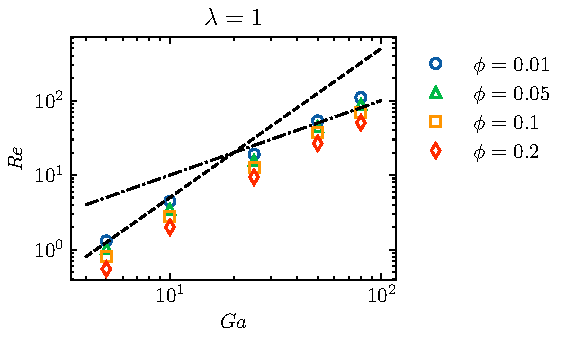
\includegraphics[height = 0.25\textwidth]{image/HOMOGENEOUS_final/CA/Re_l_1.pdf}
    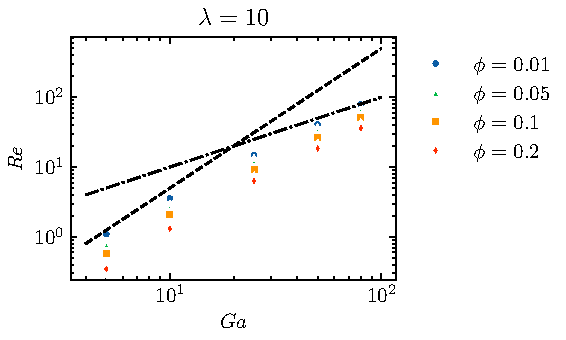
\includegraphics[height = 0.25\textwidth]{image/HOMOGENEOUS_final/CA/Re_l_10.pdf}
    \caption{
        Averaged Reynolds number based on the averaged drift velocity, $Re = \rho_f U d /\mu_f$, with $U = |\textbf{u}_p - \textbf{u}_f|$.
        $\textbf{u}_p$ and $\textbf{u}_f$ are the particle and fluid phase volume and time-averaged velocity.
        (dashed line) $Re \sim Ga^2$ (dot dashed line) $Re \sim Ga$. 
    }
    \label{fig:Reall}
\end{figure}
It is observed that for low $Ga$ the relative velocity scales approximately as $\sim Ga^2$, regardless of the volume fraction $\phi$ and viscosity ratio $\lambda$. 
Note that the \textit{Reynolds} number is globally higher for $\lambda  =1$ and $\lambda = 10$ at $Ga$ and $\phi$ fixed. 
Also, the \textit{Reynolds} number increases with decreasing volume fraction. 
Now that the global absolute kinematics are stated we can analyze pair kinematics. 

% Additionally, let us define the particle phase granular temperature or velocity fluctuation tensor as,
% \begin{equation*}
%     \avg{\delta_i \textbf{u}_i'\textbf{u}_i'}(\textbf{x},t)=
%     \frac{1}{n_p(\textbf{x},t)} 
%     \int \sum_{i}^{N_b}\delta[\textbf{x}-\textbf{x}_i(t,\FF)]  
%     \textbf{u}_i\textbf{u}_i(t,\FF)
%     d\mathscr{P}
%     - n_p \textbf{u}_p \textbf{u}_p,
% \end{equation*}
% The trace of this tensor gives us the granular temperature, namely, 
% \begin{equation*}
%     k_p = \frac{1}{2} \avg{\delta_i\textbf{u}_i'\cdot \textbf{u}_i'}-n_p\textbf{u}_p\cdot \textbf{u}_p
% \end{equation*}
% \begin{figure}[h!]
%     \centering
%     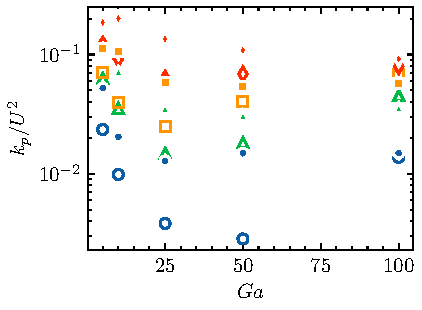
\includegraphics[height = 0.3\textwidth]{image/HOMOGENEOUS_NEW/PA/Talpha.pdf}
%     % 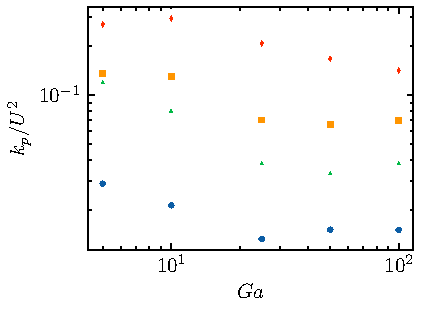
\includegraphics[height = 0.3\textwidth]{image/HOMOGENEOUS_NEW/PA/Talpha_l_10.pdf}
%     \caption{
%         Ensemble averaged granular temperature divided by the mean relative phase velocity,  $k_p = \frac{1}{2}\avg{\delta_i \textbf{u}'_i \textbf{u}_i'}/U^2$ as a function of the Galileo number.  
%         ($\pmb\bigcirc$) $\phi = 0.01$; ($\pmb\triangle$) $ \phi = 0.05$; ($\pmb\square$) $\phi = 0.1$ ($\pmb\lozenge$) $\phi = 0.2$. 
%         The hollow symbols correspond to $\lambda = 1$, the filled symbols to $\lambda = 10$.
%     }
%     \label{fig:Reall}
% \end{figure}
% We display on \ref{fig:Reall} the values of the granular temperature for all our DNS. 
% It is shown that the dimensionless granular temperature increase with $\phi$ at $\lambda$ fixed and is non-monotonic with $Ga$. 
% Additionally, one can note that The value of $k_p/U^2$ globally increase with $\lambda$. 
% The relative velocity and the granular temperature both represent an averaged representation of the particle phase kinematics. 
% The granular temperature measure indirectly the relative motion between particles however it is hard to 

\subsection{Mean age of interaction}

Now, we propose to evaluate the age distribution $P_a$ and to verify the \textit{random destruction assumption} stated in \ref{sec:Theory}. 

In \ref{fig:age_picture} we display the dimensionless age distribution $P_a(a)$, measured in our DNS. 
The age is made dimensionless using the timescale, $U/d_p$ with $d_p = n_p^{-1/3}$.
It is shown in the next few paragraphs that $d_p$ is a representative inter-droplet length scale. 
The theoretical prediction for the age distributions, $P_a(a)$, are obtained by computing the mean \textit{age} $a_p$ from our DNS and using \ref{eq:Pa}. 
The values of $a_p$ are displayed in \ref{fig:tau_p} and will be discussed hereafter. 

It is seen on \ref{fig:age_picture} (right) that the age distributions of the inertial cases are rather well represented by the theoretical age distributions from \ref{eq:Pa}.
Consequently, the \textit{random destruction assumption} holds for the inertial cases. 
Additionally, we see that the distributions spread as the volume fraction decreases.
\begin{figure}[h!]
    \centering
    % 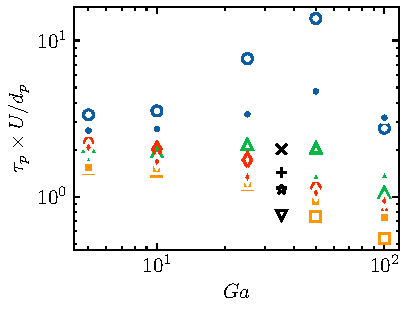
\includegraphics[height = 0.3\textwidth]{image/HOMOGENEOUS_NEW/tau_Ga.pdf}
    % 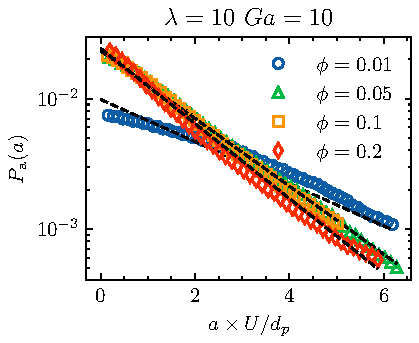
\includegraphics[height = 0.3\textwidth]{image/HOMOGENEOUS_NEW/Dist/Pa_l_10_Ga_10.pdf}
    % 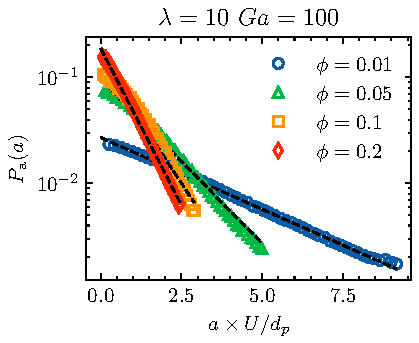
\includegraphics[height = 0.3\textwidth]{image/HOMOGENEOUS_NEW/Dist/Pa_l_10_Ga_100.pdf}
    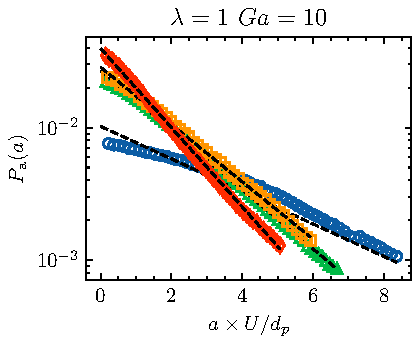
\includegraphics[height = 0.3\textwidth]{image/HOMOGENEOUS_NEW/Dist/Pa_l_1_Ga_10.pdf}
    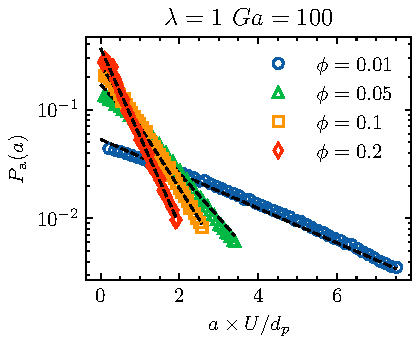
\includegraphics[height = 0.3\textwidth]{image/HOMOGENEOUS_NEW/Dist/Pa_l_1_Ga_100.pdf}
    \caption{
    Age distribution function $P_a(a)$ in terms of the dimensionless age, for $\lambda = 1$.
    (dashed lines) Theoretical age distributions, computed based on the mean age, see \ref{eq:Pa}. 
    The ages are made dimensionless using the relative velocity $U$ and the droplet length scale $d_p = n_p^{-1/3}$.  
    (right) High inertia effects ($Ga = 100$),
    (left) Low inertia effects ($Ga = 10$),
    }
    \label{fig:age_picture}
\end{figure}
In \ref{fig:age_picture} (left)  we provide the age distributions for $Ga = 10$. 
It is seen that the age distribution is well described by \ref{eq:Pa} for $\phi \le 0.05$.
However, for $\phi = 0.01$ we observe that the predicted values of $P_a$ are higher than the DNS results for small ages and smaller for high ages. 
Therefore, at low \textit{Galileo} and low $\phi$ the \textit{random destruction assumption} doesn't seem to remain valid. 
As mentioned earlier the \textit{random destruction assumption} must hold for flows with high droplet velocity fluctuations, since it induces randomness among the droplet interactions \citep{zhang2023evolution} and the interaction history is not important.  
It is clear that for $\phi \to 0$ and $Re \to 0$, the dispersed phase fluctuation also tends to $0$, making this condition harder to meet. 
No differences on $P_a$ are observed when $\lambda = 10 $ therefore we do not display the graphs. 
Anyhow, apart from the dilute and low inertia cases, it is reasonable to say that \ref{eq:Pa} is representative of the age distribution function obtained by DNS.
Consequently, according to \ref{eq:Pa} and \ref{eq:a_p2} the averaged duration of interaction is equivalent to the inverse of the mean destruction rate, that is $\tau_p = a_p$. 

Now let's investigate the value of $a_p$ for all our DNS cases. 
In \ref{fig:tau_p} we display the dimensionless mean age for all our numerical experiments. 
\begin{figure}[h!]
    \centering
    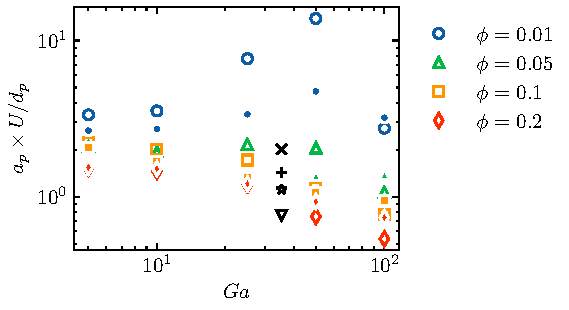
\includegraphics[height = 0.3\textwidth]{image/HOMOGENEOUS_NEW/PA/age.pdf}
    % 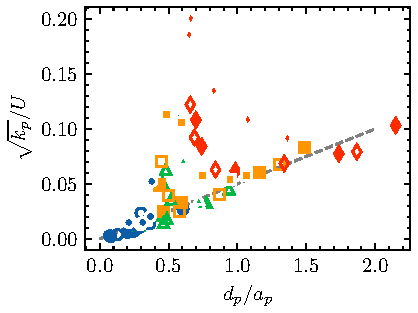
\includegraphics[height = 0.3\textwidth]{image/HOMOGENEOUS_NEW/PA/Corr.pdf}
    % 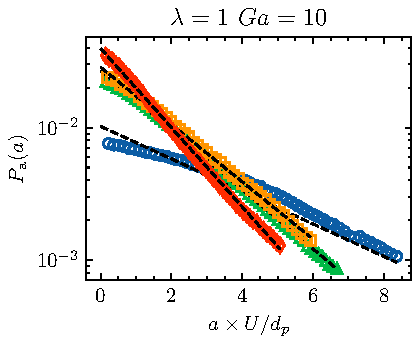
\includegraphics[height = 0.3\textwidth]{image/HOMOGENEOUS_NEW/Dist/Pa_l_1_Ga_10.pdf}
    % 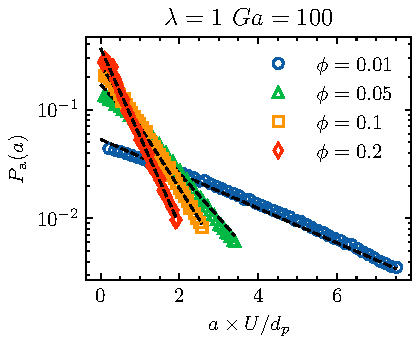
\includegraphics[height = 0.3\textwidth]{image/HOMOGENEOUS_NEW/Dist/Pa_l_1_Ga_100.pdf}
    \caption{
    (left) Mean dimensionless age $\tau_a =  \int_0^\infty aP_a(\textbf{x},t,a)da$ in terms of the \textit{Galileo} number for different volume fraction :   
    ($\pmb\bigcirc$) $\phi = 0.01$; ($\pmb\triangle$) $ \phi = 0.05$; ($\pmb\square$) $\phi = 0.1$ ($\pmb\lozenge$) $\phi = 0.2$.
    The hollow symbols correspond to $\lambda = 1$, the filled symbols to $\lambda = 10$.
    Black symbols represent the DNS results of \citet{zhang2023evolution} for hard sphere suspensions with $\phi = 0.0168,0.0565,0.1341,0.2622$, corresponding to the symbols : $\pmb\times, \pmb +, \pmb\star , \pmb\triangledown$, respectively.
    }
    \label{fig:tau_p}
\end{figure}
Let us first comment on the non-dilute cases $\phi\geq 0.05$. 
It seems that $a_p$ scales well with $U/d_p$ for this range of volume fractions since its values range between $2$ and $0.5$, which is reasonably close to $1$. 
At low volume fraction, it is observed that $a_p$ is constant with $Ga$ until $Ga = 50$ where the mean age starts to decrease. 


At low volume fraction, however, $a_p$ is higher and reaches a peak at $\phi=0.01$, $Ga=50$, $\lambda=1$.
This may be correlated with the values of $A_{xx}$ on \ref{fig:A} which also reach a maximum for these parameters. 
Indeed, since $A_{xx}$ is rather high for these simulations, we know that droplets are, on average, in a side-by-side configuration.
The information that $a_p$ is large too indicated that these sides-by-side configuration seems stable for $\lambda = 1$. 
In opposition to $\lambda = 10$ we observe smaller $a_p$ and also smaller $A_{xx}$ at $\phi = 0.01$ and $Ga = 50$, indicating that, on average, the interactions are not as long, while the microstructure is more isotropic. 

The $\pmb\times$ symbol represents DNS conducted by \citet{zhang2023evolution} on the sedimentation of solid spheres in a liquid. 
The mean age measured in their DNS seems to possess even lower $a_p$ at equivalent $\phi$ and $Ga$. 
This suggests that the duration of interaction of solid particles is shorter than the one of viscous droplets ($\lambda = 10$).
Note that the duration of interaction is even shorter for $\lambda = 1$. 
Pair interaction mechanisms have been investigated by \citet{yin2008lattice} when studying spherical bubbles and solid particle suspensions.
They reach the conclusion that the weaker wake generated by bubbles tends to make them spend more time in close horizontal orientations, in opposition to solid spherical particles. 
Thus, this finding strongly supports the previous observation since the mean age for solid particles is lower than for $\lambda = 1$ indicating that the interactions are less stable for the former. 
In summary, the mean age of interaction seems to be a good way to measure the droplet pairs stability since it provides a way to measure their interaction time. 
This time is shorter for increasing $\phi$, and non-monotonic with $\lambda$ and $Ga$. 
And, in the dilute regime ($\phi = 0.01$) $a_p$ seems to decrease with increasing $\lambda$. 

\subsection{Droplets normal approach velocity}

In the next section we will be interested in the velocity fields $\textbf{w}_p^\text{nst}(\textbf{x},\textbf{r},t,a)$ since it appears in the source term $\textbf{W}(\textbf{x},t)$, which is at the origin of the modifications of the microstructure, see \ref{eq:dt_R}. 
To give a simpler representation of $\textbf{w}_p^\text{nst}(\textbf{x},\textbf{r},t,a)$, we first study the normal approach velocity averaged on all relative positions $\textbf{r}$, that is,  
\begin{equation*}
    w_{pn}^aP_a(\textbf{x},t,a)
    = \frac{1}{n_p(\textbf{x},t)}
    \int_{\mathbb{R}^3}
    \frac{\textbf{r}}{r} \cdot \textbf{w}^\text{nst}_p
    P_\text{nst}(\textbf{x},\textbf{r},t,a) d\textbf{r}.
\end{equation*}
In this way, $w^\text{a}_{pn}(\textbf{x},t,a)$ is the average relative normal approach velocity between the nearest pair of droplets of age $a$. 
The superscript $^a$ indicates that $w_{pn}^a$ is conditioned only on the age $a$. 
It represents the average approach velocity from one droplet to its nearest neighbor, measured from the time when the droplets became nearest neighbors, $a=0$.
A sketch of what we mean by ``normal approach relative velocity'' is given \ref{fig:normal_vel_picture} (right). 
\begin{figure}[h!]
    \centering
    % 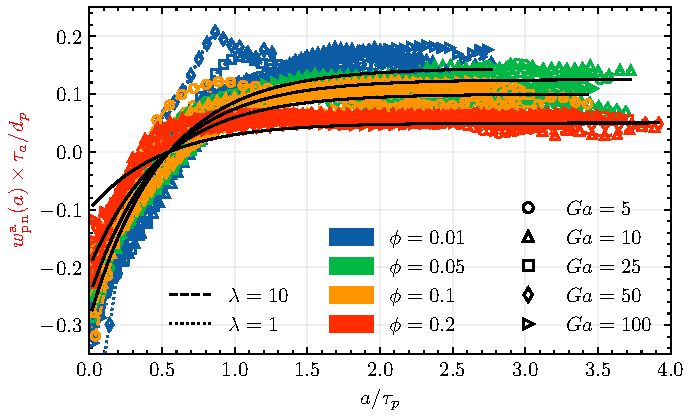
\includegraphics[height = 0.4\textwidth]{image/HOMOGENEOUS_NEW/Age_cond/uR_rel.pdf}
    % \includegraphics[height = 0.3\textwidth]{image/HOMOGENEOUS_NEW/Age_cond/r_l_10_PHI_10.pdf}
    \begin{tikzpicture}[ scale = 0.6]
        \node (img) at (-0.7\textwidth,0){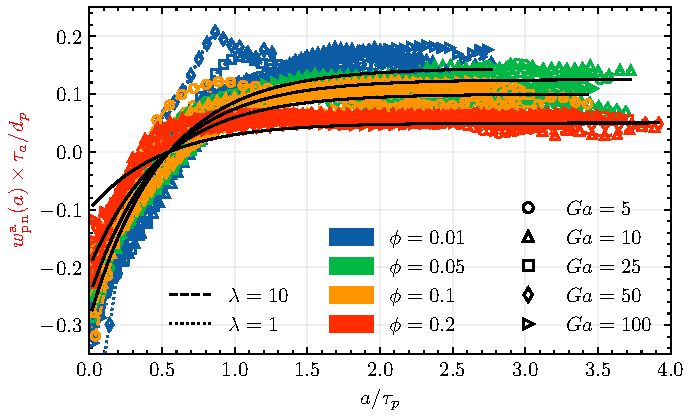
\includegraphics[height = 0.4\textwidth]{image/HOMOGENEOUS_NEW/Age_cond/uR_rel.pdf}};
        \filldraw[ gray!50!white](0,0) circle (0.5);
        \filldraw[ gray!50!white](1,3)circle (0.5);
        % \draw[fill=gray,opacity=0.2](5,-0.2)circle (0.5);
        % \draw[fill=gray,opacity=0.2](-3,2)circle (0.5);
        % \draw[fill=gray,opacity=0.2](-5,0.2)circle (0.5);
        \draw(0,0)node[right]{$\textbf{x}_i$};
        \draw[dashed](0,0)--(1,3)node[right]{$\textbf{x}_j$};
        % \draw[very thick,<-,blue](-1,0)--++(0,1)node[right]{$\bm{b}$};
        \draw[very thick,->](1,3)--++(0.9,-1.8)node[above right]{$\textbf{w}^\text{nst}(a)$};
        \draw[very thick,->,red](1,3)--++(-0.5,-1.5)node[left]{$w_{ij,n}(a)$};
        \draw[dashed](1,3)++(0.9,-1.8) -- (1,3)++(-0.5,-1.5);
        \node (ii) at (1,-1){$\textbf{w}_{ij} = \textbf{u}_j - \textbf{u}_i$};
        \node (ii) at (1,-1.6){$w_{ij,n} = \textbf{w}_{ij}\cdot \textbf{r}/|\textbf{r}|$};
        % \draw[very thick,->](0,0)--++(1,0)node[below right]{$\bm{e_x}$};
        % \draw[very thick,->](0,0)--++(0,1)node[left]{$\bm{e_y}$};
        % \draw(3,1)++(199:1)node[above left]{$\beta$} arc(199:159:1);
        % \draw(0,0)++(0:1)node[above right]{$\theta$} arc(0:20:1);
    \end{tikzpicture} 
    \caption{(left) Relative normal approach velocity between two nearest neighbors, averaged conditionally on the age of interaction.  
    The age $a$, as well as the velocity are made dimensionless  with the mean age $\tau_a$ and the length scale $d_p = n_p^{-1/3}$. 
    % The symbols represent the different \textit{Galileo} numbers, the colors the different 
    % ($\pmb\bigcirc$) $Ga=10$; ($\pmb\triangle$) $ Ga = 25$; ($\pmb\square$) $Ga = 50$ ($\pmb\lozenge$) $Ga =100$.
    % The colors represent the different volume fractions, (blue) $\phi =0.01$, (green) $\phi = 0.05$ (organ) $\phi=0.1$ (red) $\phi = 0.2$. 
    % The white symbols correspond to $\lambda = 1$, and black symbols to $\lambda = 10$. 
    (right)
    Sketch of two nearest neighbors with their position $\textbf{x}_i$ and $\textbf{x}_j$, velocities $\textbf{u}_{i}$ and $\textbf{u}_j$, relative velocity $\textbf{w}_{ij}$ and normal relative velocity $w^{ij,n}$. 
    (black lines) Semi-empirical formulation \eqref{eq:semi-emprical_fits}.
    }
    \label{fig:normal_vel_picture}
\end{figure}
The approach velocity $w_{pn}^a(\textbf{x},t,a)$ for all the DNS carried in this work is displayed \ref{fig:normal_vel_picture} (left). 
The x-axis is made dimensionless with the averaged duration of interaction, $\tau_p$, and the y-axis is scaled with the velocity scale $d_p /\tau_p$. 
At early ages, we observe that $w_{pn}^a<0$.
Then it eventually reaches zero for  $a \approx 0.5\tau_p$.
After this time $w_{pn}^a>0$ and remains constant with respect to $a$. 
Hence, on average, droplets approach each other at early ages ($w_{pn}^a<0$), and then they move apart for $a > \tau_p$ with a constant average velocity.

Two important features are identified from \ref{fig:normal_vel_picture} (left).
First, all curves are roughly similar, even if we can see slight differences in magnitude for the different $\phi$. 
Thus, regardless of the flow parameters, $w_{pn}^a(\textbf{x},t,a)$ scale roughly as $d_p /\tau_p$. 
Second,  $w_{pn}^a(\textbf{x},t,a)$ seems to relax for age, $a > \tau_p$, to reache a constant positive value. 
Consequently, we demonstrated that $\tau_p$ and $d_p$ were the correct time and length scales which govern the inter-droplet scale kinematics, and that $\tau_p$ is also the relaxation time of $w_{pn}^a(\textbf{x},t,a)$. 
In general, we believe that $w_{pn}^a(\textbf{x},t,a)$ may be useful for future studies aiming to construct models based on the relative velocity between droplets \citep{rao2008introduction}. 


We would now like to build a kinetic model for the normal approach velocity of droplets. 
This is of particular interest since closure terms such as collision kernel are directly related to the normal approach velocity between droplets \citep{sundaram1997collision}.
Looking at \ref{fig:normal_vel_picture} we can propose that the normal approach velocity has the form:
\begin{equation}
    w_{pn}^a(\textbf{x},t,a) = \frac{d_p}{\tau_p} \left(
        - C_1 e^{- 2 a/\tau_p }
        + C_2
    \right)
\end{equation}
The theoretical observations made in \ref{sec:Theory} suggest that in a statistically steady-state regime, the normal approach velocity must respect the condition :
\begin{equation}
\int_\mathbb{R} w_{pn}^aP_a(\textbf{x},t,a) da = 0 
\end{equation}
which means that both constants must respect $C_2 = C_1 /3$. 
% Let consider that the maximum value of $w_{pn}^a$ is reached for the lowest volume fraction $\phi = 0.01$ at $a \to \infty$ (see \ref{fig:normal_vel_picture}).     
% Besides approaching the packing volume fraction limit $\phi_\text{max}$ the relative velocity must approach zero. 
Additionally, suppose that $w_{pn}^a(\textbf{x},t,a\to\infty,\phi)$ varies linearly with $\phi$ from $w_{pn}^a(\textbf{x},t,a\to\infty,\phi = 0.01) \approx 0.15$ to $w_{pn}^a(\textbf{x},t,a\to\infty,\phi = 0.2) \approx 0.05$. 
This leads us to $C_2 \approx -1/2 (\phi - 0.01) + 0.01$. 
Note that the dependency of $w_{pn}$ on $Ga$ and $\lambda$ is implicitly included in the mean age.
Making use of all these remarks a consistent model for the relative normal approach velocity is, 
\begin{equation}
    w_{pn}^a(\textbf{x},t,a) = \frac{d_p}{\tau_p} 
    \left(
        0.15
        -\frac{\phi}{2}
    \right)\left(
        1 - 3e^{-2a/\tau_p}
    \right).
   \label{eq:semi-emprical_fits}
\end{equation}
On \ref{fig:normal_vel_picture}, we can observe that the black lines, representing \ref{eq:semi-emprical_fits} for various values of $\phi$, describe relatively well the mean normal approach velocity measured in the DNS. 
Thus, we obtained a reasonable model for $w_{pn}$ in terms of the volume fraction and the mean age of interaction $\tau_p$.
The remaining thing to do would be to create a closed model for $\tau_p$ in terms of $Ga$, $\phi$ and $\lambda$. 



\subsection{Relative particles kinematic}

In the previous sections we have seen that the timescale governing both, the microstructure evolution and the particles pair relative velocity is $\tau_p$.   
We now give a visual representation of the nearest pair relative velocity in space to better understand how the relative kinematic behave.  
To that end we compute the nearest relative velocity and age, averaged on all ages, that is,
\begin{align*}
    \textbf{w}^\text{r}_pP_r(\textbf{x},\textbf{r},t)
    =\int_0^\infty \textbf{w}^\text{nst}_pP_\text{nst}(\textbf{x},\textbf{r},t,a) da,\\
    a^rP_r(\textbf{x},\textbf{r},t)
    =\int_0^\infty a P_\text{nst}(\textbf{x},\textbf{r},t,a) da.
\end{align*}
The superscript $^\text{r}$ indicate that the quantity $\textbf{w}^\text{r}_p$ and $a^r$ is conditioned on the relative position \textbf{r} only.
As will be demonstrated, having a good estimation of these velocities and ages mean fields allows one to reconstruct the history of the particles' kinematic interactions. 
To be able to visualize
$\textbf{w}^\text{r}_p(\textbf{x},\textbf{r},t)$
and 
$a^r(\textbf{x},\textbf{r},t)$
on 2D plots we consider an axis symmetry along the vertical axis, and average the values of 
$\textbf{w}^\text{r}_p(\textbf{x},\textbf{r},t)$
and $a^r(\textbf{x},\textbf{r},t)$
on the polar coordinate, as it has been done for $P_\text{nst}$ in \ref{sec:microstructure}. 
However, unlike in \ref{sec:microstructure} we do not assume symmetry with respect to the horizontal plane. 

\subsubsection{Impact of the inertial effects}

The first effect that we study is the impact of the inertial effects on the particles relative kinematic.  
In \ref{fig:Why_Ga_matter} we display the velocity fields $\textbf{w}_p^r$ represented by the arrows that are colored by the mean dimensionless age $a^r$.  
On the left panel, we observe a low inertial case ($Ga = 10$), while on the right panel, we display a highly inertial case ($Ga=100$), both for $\lambda =1$ and $\phi=0.05$.
\begin{figure}[h!]
    \centering
    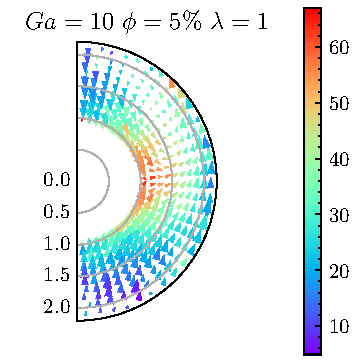
\includegraphics[height=0.35\textwidth]{image/HOMOGENEOUS_NEW/Dist/U_rel_l_1_Ga_10_PHI_5.pdf}
    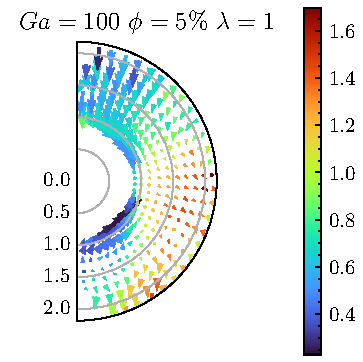
\includegraphics[height=0.35\textwidth]{image/HOMOGENEOUS_NEW/Dist/U_rel_l_1_Ga_100_PHI_5.pdf}
    % \begin{tikzpicture}[scale=0.8]
    %     \filldraw[ gray!50!white](0,0) circle (0.5);
    %     \filldraw[ gray!50!white](1,3)circle (0.5);
    %     \filldraw[ gray!50!white](-0.2,3.5)circle (0.5);
    %     % \draw[fill=gray,opacity=0.2](5,-0.2)circle (0.5);
    %     % \draw[fill=gray,opacity=0.2](-3,2)circle (0.5);
    %     % \draw[fill=gray,opacity=0.2](-5,0.2)circle (0.5);
    %     \draw(0,0)node[right]{$p_1, \; \textbf{x} = 0 $};
    %     \draw[dashed](0,0)--(1,3)node[right]{$p_2, \;\textbf{x}+\textbf{r}$};
    %     \draw[dashed](-0.2,3.5)node[right]{$p_3$};
    % \end{tikzpicture} 
    % 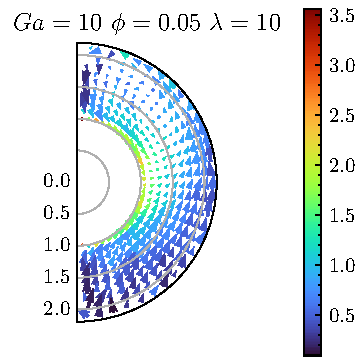
\includegraphics[height=0.35\textwidth]{image/HOMOGENEOUS_NEW/Dist/U_rel_l_10_Ga_10_PHI_5.pdf}
    % 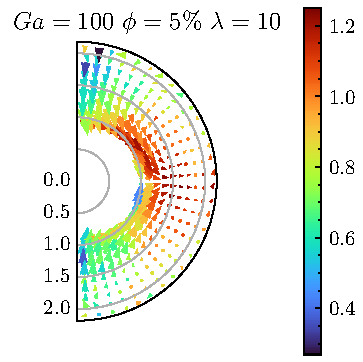
\includegraphics[height=0.35\textwidth]{image/HOMOGENEOUS_NEW/Dist/U_rel_l_10_Ga_100_PHI_5.pdf}
    \caption{
         Quiver plots of the relative averaged velocity field $\textbf{w}^\text{r}(\textbf{x},\textbf{r},t)$ colored by the averaged dimensionless age $a^r(\textbf{x},\textbf{r},t)$ for $\phi = 0.05$ and $\lambda +1$.
         (left) $Ga = 10$ (right) $Ga =100$. }
    \label{fig:Why_Ga_matter}
\end{figure}

The first aspect that we would like to clarify is the non fore-aft symmetry of the velocity fields $\textbf{w}_p^\text{nst}$ with respect to the horizontal plane. 
Indeed, in plots display on \ref{fig:Why_Ga_matter} we remark that the $\textbf{w}_p^\text{nst}$ exhibit a clear asymmetry with respect to the horizontal plane.
This is explained by the non commutativity of the function $h_{ij}$ in the indices $i$ and $j$ in \ref{eq:q_nstij}, as a result $\textbf{w}_p^r(\textbf{x},t,r,\theta) \neq \textbf{w}_p^r(\textbf{x},t,r,-\theta)$. 
Indeed, as it is depicted on \ref{fig:diagram_asym}, in the cases were the neighboring nearest particle is far from the test particle, the chance for this particle to have another nearest neighbor which is closer is high. 
Thus, the nearest neighbor of the nearest neighbor of the test particle, is not necessarily the test particle. 
This induces asymmetry in the nearest neighbor statistics. 
That explains why the plots on \ref{fig:Why_Ga_matter} are not symmetrical when we observe the fields at sufficiently large distance $|\textbf{r}|$. 
Note that this asymmetry would not be present if we had considered classic particle pair average as it is done in \cite{shajahan2023inertial}. 
To summaries, in the situation where we observe $\textbf{w}_p^r$ for large $|\textbf{r}|$ the test particle can be considered as being \textit{isolated}, as its nearest neighbor is at a large distance $|\textbf{r}|$ from the test particle. 
Additionally, the nearest neighboring particle, if located far enough, has 
potentially a nearest neighbor that is closer than the test sphere, as explained on \ref{fig:diagram_asym}. 
Consequently, provided that the nearest neighbor of the test sphere is far enough, we can be sure that on average it approaches a pair of particles or more, that are packed together. 

\begin{figure}[h!]
    \centering
    \hfill
    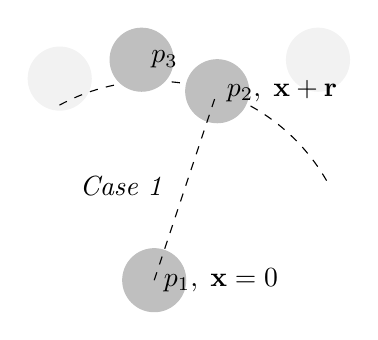
\begin{tikzpicture}[scale=0.8]
        \filldraw[ gray!10!white](+2.6,3.5)circle (0.5);
        \filldraw[ gray!10!white](-1.5,3.2)circle (0.5);
        \draw[dashed](30:3.16) arc (30:120:3.16);
        \filldraw[ gray!50!white](0,0) circle (0.5);
        \filldraw[ gray!50!white](1,3)circle (0.5);
        \filldraw[ gray!50!white](-0.2,3.5)circle (0.5);
        \draw(0,0)node[right]{$p_1, \; \textbf{x} = 0 $};
        \draw[dashed](0,0)--(1,3)node[right]{$p_2, \;\textbf{x}+\textbf{r}$};
        \draw[dashed](-0.2,3.5)node[right]{$p_3$};
        \node[ultra thick] (title) at (-0.5,1.5) {\textit{Case 1}};
    \end{tikzpicture} 
    \hfill
    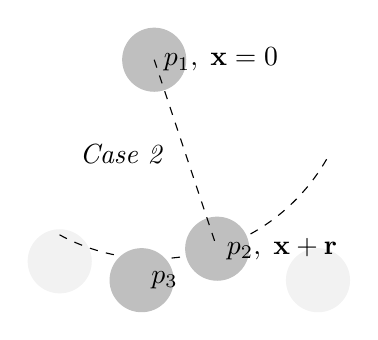
\begin{tikzpicture}[rotate=180, xscale=-0.8,yscale=0.8]
        \filldraw[ gray!10!white](+2.6,3.5)circle (0.5);
        \filldraw[ gray!10!white](-1.5,3.2)circle (0.5);
        \draw[dashed](30:3.16) arc (30:120:3.16);
        \filldraw[ gray!50!white](0,0) circle (0.5);
        \filldraw[ gray!50!white](1,3)circle (0.5);
        \filldraw[ gray!50!white](-0.2,3.5)circle (0.5);
        \draw(0,0)node[right]{$p_1, \; \textbf{x} = 0 $};
        \draw[dashed](0,0)--(1,3)node[right]{$p_2, \;\textbf{x}+\textbf{r}$};
        \draw[dashed](-0.2,3.5)node[right]{$p_3$};
        \node[ultra thick] (title) at (-0.5,1.5) {\textit{Case 2}};
    \end{tikzpicture} 
    \hfill
    % \begin{tikzpicture}[scale=0.8]
    %     \filldraw[ gray!10!white](+2.6,3.5)circle (0.5);
    %     \filldraw[ gray!10!white](-1.5,3.2)circle (0.5);
    %     \draw[dashed](-30:3.16) arc (-30:-120:3.16);
    %     \filldraw[ gray!50!white](0,0) circle (0.5);
    %     \filldraw[ gray!50!white](1,-3)circle (0.5);
    %     % \filldraw[ gray!20!white](-1.4,-3.3)circle (0.5);
    %     \filldraw[ gray!50!white](-0.2,-3.5)circle (0.5);
    %     % \draw[fill=gray,opacity=0.2](5,-0.2)circle (0.5);
    %     % \draw[fill=gray,opacity=0.2](-3,2)circle (0.5);
    %     % \draw[fill=gray,opacity=0.2](-5,0.2)circle (0.5);
    %     \draw(0,0)node[right]{$p_1, \; \textbf{x} = 0 $};
    %     \draw[dashed](0,0)--(1,-3)node[right]{$p_2, \;\textbf{x}+\textbf{r}$};
    %     \draw[dashed](-0.2,-3.5)node[right]{$p_3$};
    %     \node[ultra thick] (title) at (-0.5,-1.5) {$Case\; 2$};
    % \end{tikzpicture} 
    \caption{
        Diagram that highlights the asymmetry of the nearest pair statistic when the nearest neighbor is relatively far from the test particle.
        (\textit{Case 1}) Particle $p_1$ with  its nearest neighbor, $p_2$, located at the \underline{top} of it. 
        (\textit{Case 2}) Particle $p_1$ with  its nearest neighbor, $p_2$, located at the \underline{bottom} of it. 
        (\textit{Case 1} and \textit{2})
        In these situations the particle $p_2$ located at $\textbf{x} + \textbf{r}$, is the nearest neighbor of the particle $p_1$ located at $\textbf{x}$. 
        Since $|\textbf{r}|/d$ is assumed to be large, the nearest neighbor of the particle $p_2$ is more likely to be another nearest neighbor than $p_1$ such as the particle $p_3$, which is closer.
        This is due to the rapid decay of $P_\text{nst}$ for large $|\textbf{r}|/d$, see \ref{fig:Pnst_high_Ga}. 
        In these cases the nearest neighbor of $p_1$ is $p_2$, but the contrary is not true, inducing asymmetry in the statistics.  
    }
    \label{fig:diagram_asym}
\end{figure}

Now that this issue has been clarified, we can proceed to interpret the plots in \ref{fig:Why_Ga_matter}.
The beginning of the interactions happen at the early ages, meaning in the dark blue areas in  \ref{fig:Why_Ga_matter}, which are located on the top or bottom of the particle of reference.
The ending of the interactions corresponds to the greater ages, which are represented by the red areas. 
As shown by \ref{fig:Why_Ga_matter} (left), at low \textit{Galileo} number the nearest particle has a tendency to come from the top or bottom and leave through the sides. 
If the nearest particle is at a reasonable distance $|\textbf{r}| < 1.5d$ on the sides of the test particle, we can see that the vertical relative velocity is on average null, but positive in the radial component.
In this area, the age is at its maximum (dark red zone), therefore the interaction come to an end, meaning that the nearest particles get replace by another. 
Note that for the particles at a larger distance of the test particle, say $|\textbf{r}|>2$, have an averaged positive vertical relative velocity. 
As discussed above, in this situation the neighbor on the side is more likely to be closer to another particle. 
Consequently, if the test particle is isolated, with neighboring particles sufficiently far on the side, it will rise on average with a lower velocity than the latter particles.
Thus, particles at contact  seems to get apart because of the non-null radial velocity, and particle at distance seems to get apart because of the non-null vertical velocity.  
Consequently, on average the side-by-side configuration is not stable in this case, which partly explains why the particle distribution doesn't form any layer or such oriented microstructure at these $Ga$.   

% A plausible explanation for this phenomenon is that the leading particle accelerate the trailing particle with its wake on a first stage. 
% Then, the trailing particle arise to the same altitude as the leading particle, but still goes faster than the leading particle due to the acceleration provided by the wake of the latter particle.
% If the particles get in contact then the interaction duration seem to last longer, and the particles might even get trap in a small stagnation zone on the side of the particles.


For high \textit{Galileo} number, see \ref{fig:Why_Ga_matter} (right), the relative averaged velocity is nearly null on the sides and below the test particle. 
It is a statistical representation, meaning that, $\textbf{w}_p^r = 0$, just witnesses of the fact that the particles' relative velocity are not correlated with the relative position in this area. 
Thus, it is hard to say if the area where $\textbf{w}_p^r = 0$ corresponds to actual stagnation zones where both particles are in equilibrium, or if the relative velocity is just not correlated. 
Additionally, the particles at a large distance on the top of the test particle have a downward velocity. 
Meaning that if the test sphere is isolated and approach one or several  particles on the top of it (see \ref{fig:diagram_asym} (\textit{Case 1})), it will eventually catch up the latter particles. 
On the contrary, if the particle is isolated and that the nearest neighbor is at the bottom (see \ref{fig:diagram_asym} (\textit{Case 2})), the velocity is either pointing downward, or it is not correlated with the position, as indicated by the magnitude of $\textbf{w}_p^r$. 
A plausible explanation for this phenomenon is that the reference particle, when being isolated, goes faster than the potentially packed nearest neighbor.
Therefore, the test sphere can either catch up with the nearest particle if it is above, or move further away from it if it is below.
Also, it is interesting to notice that in this case the particles at near contact on the bottom of the test particles results from early interaction, denoted by the dark blue zone. 
It can be interpreted as follows : since 
initial time of interaction is on average low in this zone, it does mean that particles replace an old nearest neighbor that where at near contact of the test particles. 
Thus, in this case the nearest neighbor reaches the test sphere which were rising slowly because of a potentially close neighbor. 

Ultimately, the fields $\textbf{w}^r_p(\textbf{x},\textbf{r}, a)$ provide a quantitative averaged representation of what is known as the \textit{Drafting Kissing Tumbling} \citep{fortes1987nonlinear} mechanism. 
Indeed, in both case particles eventually approach from the verticals (\textit{Drafting}), nearly touch each other (\textit{Kissing}), and leave through the sides (\textit{Tumbling}). 
Statistically, the \textit{Tumbling} part is not present in the high inertial case, which  explains the creation of anisotropic structures or more stable side-by-side configurations. 
For bubble pair interactions \citet{zhang2021three} observed such DKT behavior.
They also reported side-by-side stable configuration of pairs. 
However, at same \textit{Galileo} than  \citet{zhang2021three} ($Ga = 10$) we were not able to identify this pair mechanism. 


To support the deduction made above, we displayed in \ref{fig:unst_ga} the absolute conditioned averaged center of mass velocity of the test sphere, defined as,
\begin{equation*}
    \textbf{u}^\text{r}_p(\textbf{x},\textbf{r},t)  
    =
    \frac{1}{P_r(\textbf{x},\textbf{r},t)}
    \int_0^\infty \textbf{u}^\text{nst}_pP_\text{nst}(\textbf{x},\textbf{r},t,a) da
\end{equation*}
In \ref{fig:unst_ga} (left) we clearly see that the magnitude of the test particle's vertical velocity is higher than the particle phase vertical velocity $\textbf{u}_p$ when the nearest neighbor is at near contact to the test particle, either above or below.
\begin{figure}[h!]
    \centering
    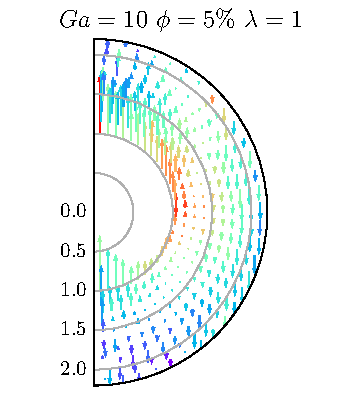
\includegraphics[height=0.35\textwidth]{image/HOMOGENEOUS_NEW/Dist/U_l_1_Ga_10_PHI_5.pdf}
    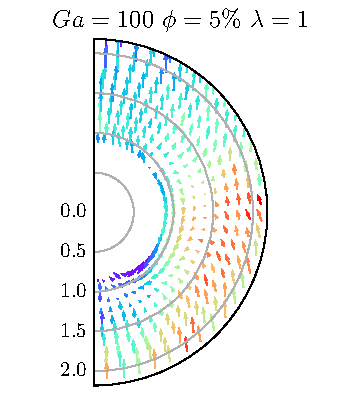
\includegraphics[height=0.35\textwidth]{image/HOMOGENEOUS_NEW/Dist/U_l_1_Ga_100_PHI_5.pdf}
    \caption{
         Quiver plots of the conditioned particle velocity field $\textbf{u}^\text{r}(\textbf{x},\textbf{r},t)$ colored by the averaged dimensionless vertical velocity difference : $(\textbf{u}^\text{r} - \textbf{u}_p )/ \textbf{u}_p$, for $\lambda = 1$ and $\phi = 0.05$. 
         (left) Low \textit{Galileo} number $Ga = 10$.
        (right) High \textit{Galileo} number $Ga = 100$.
         }
    \label{fig:unst_ga}
\end{figure}
When the nearest neighbor is at large distance of the test particle, its average velocity is lower than $\textbf{u}_p$. 
At high inertia however, the test particle velocity is higher when being isolated than with its neighbor at near contact. 
Additionally, we can see that when the particle is on the side at near contact or below, the test sphere's velocity  is lower than the mean. 
In brief in the case of $Ga = 10$ it seems that isolated particles goes slower than close neighbors packed together. 
While at higher \textit{Galileo} number it is the opposite, we observe that isolated particles  goes faster than packed neighbor. 


\subsubsection{The volume fraction dependency}
As it has been observed in \ref{fig:A} the effect of increasing $\phi$ is that it makes the particle distribution slightly more isotropic for $\phi >0.1$. 
\begin{figure}[h!]
    \centering
    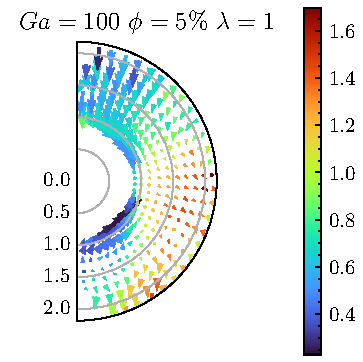
\includegraphics[height=0.35\textwidth]{image/HOMOGENEOUS_NEW/Dist/U_rel_l_1_Ga_100_PHI_5.pdf}
    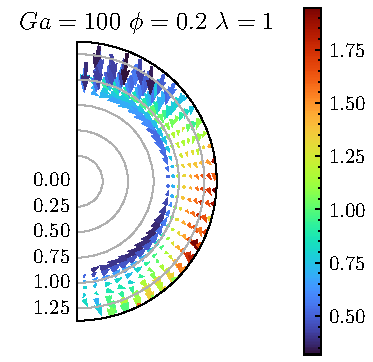
\includegraphics[height=0.35\textwidth]{image/HOMOGENEOUS_NEW/Dist/U_rel_l_1_Ga_100_PHI_20.pdf}
    % 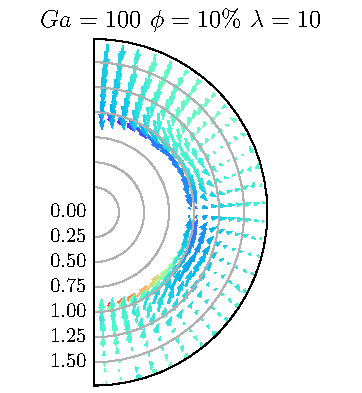
\includegraphics[height=0.35\textwidth]{image/HOMOGENEOUS_NEW/Dist/U_rel_l_10_Ga_100_PHI_10.pdf}
    % 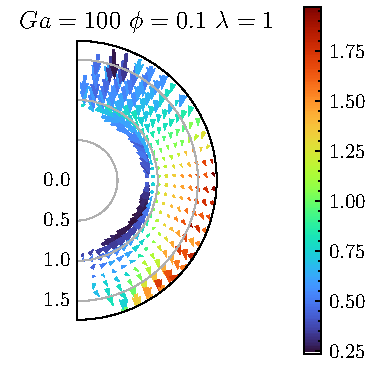
\includegraphics[height=0.35\textwidth]{image/HOMOGENEOUS_NEW/Dist/U_rel_l_1_Ga_100_PHI_10.pdf}
    \caption{Quiver plots of the relative averaged velocity field $\textbf{w}^\text{r}(\textbf{x},\textbf{r},t)$ colored by the averaged dimensionless age $a^r(\textbf{x},\textbf{r},t)$, for $Ga = 100$ and $\lambda = 1$. 
    (left) Low \textit{Galileo} number $\phi = 0.05$.
    (right) High \textit{Galileo} number $\phi = 0.2$. }
    \label{fig:Why_Phi_matter}
\end{figure}
In \ref{fig:Why_Phi_matter} we expose two situations with various volume fractions. 
In both graph we observe the same trend, despite the changes in length scales, which are due to the variations in volume fraction. 
Indeed, the stagnation zones with dark red color and the particle resulting from short interactions, dark blue color, are located approximately at the same location. 
We still observe the fore-aft asymmetry with respect to the horizontal plane, as it was discussed above. 
For other $\lambda$ and $Ga$ no particular differences could be observed with varying $\phi$. 
Overall, even if small differences might be present, the change in volume fraction doesn't seem to affect the relative kinematic of interaction between particles. 

\subsubsection{Influence of the viscosity ratio}

Lastly, we turn our attention to the effect of the viscosity ratio on pair relative kinematic.
The question that we are trying to answer is : why does a smaller viscosity ratio increase the anisotropy of the tensor $\textbf{R}(\textbf{x},t)$ as it is shown in \ref{fig:A}. 
With this objective in mind, we compare two cases at $Ga = 100$ and $\phi =0.05$, where we observe a clear difference between the distributions (see \ref{fig:Pnst_high_Ga}) between $\lambda = 1$ and $\lambda = 10$.
\begin{figure}[h!]
    \centering
    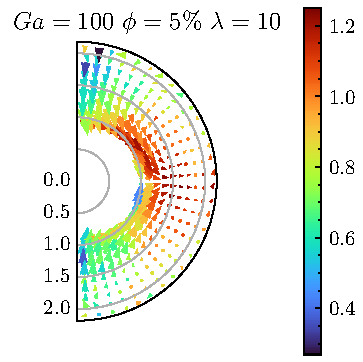
\includegraphics[height=0.35\textwidth]{image/HOMOGENEOUS_NEW/Dist/U_rel_l_10_Ga_100_PHI_5.pdf}
    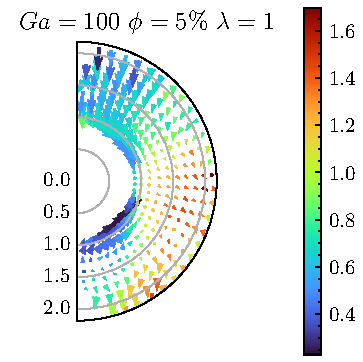
\includegraphics[height=0.35\textwidth]{image/HOMOGENEOUS_NEW/Dist/U_rel_l_1_Ga_100_PHI_5.pdf}
    % 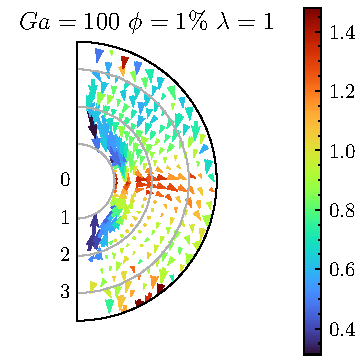
\includegraphics[height=0.35\textwidth]{image/HOMOGENEOUS_NEW/Dist/U_rel_l_1_Ga_100_PHI_1.pdf}
    % 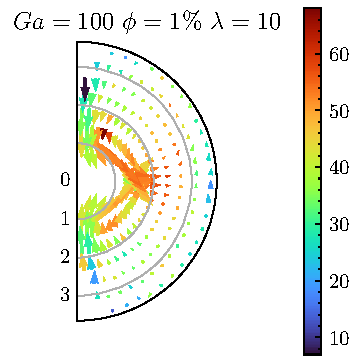
\includegraphics[height=0.35\textwidth]{image/HOMOGENEOUS_NEW/Dist/U_rel_l_10_Ga_100_PHI_1.pdf}
    \caption{Quiver plots of the relative averaged velocity field $\textbf{w}^\text{r}(\textbf{x},\textbf{r},t)$ colored by the averaged dimensionless age $a^r(\textbf{x},\textbf{r},t)$, for $\phi = 0.05$ and $Ga = 100$. 
    (left) High viscosity ratio $\lambda = 10$.
    (right) Low viscosity ratio, $\lambda = 1$. }
    \label{fig:Why_l_matter}
\end{figure}
As in the previous cases, it is clear that for both cases in \ref{fig:Why_l_matter} the neighboring particle approach on the vertical direction and end up its course on the sides.
As discussed previously, the case on \ref{fig:Why_l_matter} (right) exhibit a clear stagnation zone and asymmetry on a vertical plane. 
On the other hand for $\lambda =10$ the relative velocity on the vicinity of the particle seem to be on average positive in the radial direction. 
In addition, The asymmetry aforementioned is not present in this case. 
As discussed in the previous paragraph, and explained by \ref{fig:diagram_asym}, the presence of the skew asymmetry in the fields $\textbf{w}_p^\text{r}$ about horizontal plane, witnesses for interactions of the isolated particles clusters of particles.
The absence of such asymmetry implies the absence of such interactions, indicating that the particles are more evenly spread. 

As before, it is interesting to investigate the value of the conditional velocity $\textbf{u}^r_p$ to better understand the particles collective interactions. 
Thus, \ref{fig:unst_l} display the fields  $\textbf{u}_p^\text{r}$ for both cases. 
\begin{figure}[h!]
    \centering
    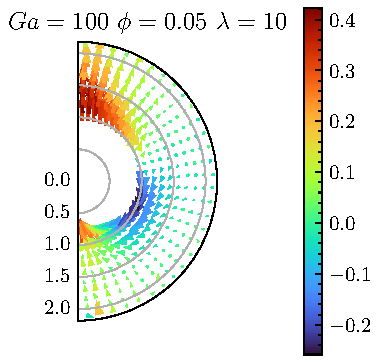
\includegraphics[height=0.35\textwidth]{image/HOMOGENEOUS_NEW/Dist/U_l_10_Ga_100_PHI_5.pdf}
    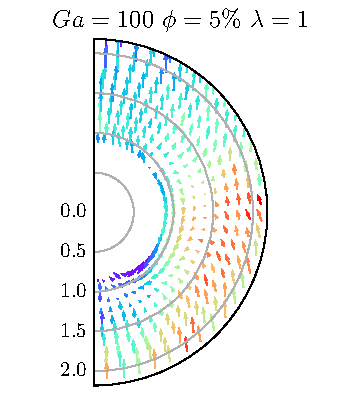
\includegraphics[height=0.35\textwidth]{image/HOMOGENEOUS_NEW/Dist/U_l_1_Ga_100_PHI_5.pdf}
    \caption{
         Quiver plots of the conditioned particle velocity field $\textbf{u}^\text{r}(\textbf{x},\textbf{r},t)$ colored by the averaged dimensionless vertical velocity difference : $(\textbf{u}^\text{r}_p - \textbf{u}_p )/ \textbf{u}_p$, for $\phi = 0.05$ and $Ga = 100$. 
         (left) High viscosity ratio $\lambda = 10$.
         (right) Low viscosity ratio, $\lambda = 1$.
         }
    \label{fig:unst_l}
\end{figure}
On \ref{fig:unst_l} (left) we first notice that $\textbf{u}^\text{r}(\textbf{x},\textbf{r},t)$ behave similarly as the low inertial case display on \ref{fig:unst_ga} (left).
However, for $\lambda = 10$, the isolated particles' velocity is roughly equal to $\textbf{u}_p$. 
If isolated particle rise at the average velocity it is because the isolated particles constitute the majority of the realization since the trace of \textbf{R} is rather high, see \ref{fig:A}.
Therefore, this fact is not particularly relevant as it is just a statistical bias. 
Nevertheless, we can still conclude that for $\lambda = 10$ particles goes faster with a nearest neighbor on top or bottom, while for  $\lambda = 1$ particles goes faster when the nearest neighbor is at large distance. 

\subsubsection{Relation with the particle phase velocity fluctuation tensor}

In addition to provides physical explanation the field $\textbf{u}_p^d = \textbf{u}^r_p - \textbf{u}_p$ is of great importance to study the particle phase fluctuation tensor $\avg{\delta_i \textbf{u}_i' \textbf{u}_i'}$ which is of crucial importance in multiphase flow modeling. 
Indeed, it can be shown that 
\begin{equation*}
    \frac{\avg{\delta_i \textbf{u}_i' \textbf{u}_i'}}{n_p}(\textbf{x},t)
    =  
    \int_{\mathbb{R}^3 }
    \textbf{u}_p^d
    \textbf{u}_p^d
    P_{nst}(\textbf{r}|\textbf{x},t)
    d\textbf{r}
    + \int_{\mathbb{R}^3 }
    \textbf{F}(\textbf{r},\textbf{x},t)
    d\textbf{r}
\end{equation*}
where, $\textbf{F} = \avg{\sum_i\sum_{j\neq i}\delta_j\delta_i h_{ij}(\textbf{u}_i - \textbf{u}_p^{nst})(\textbf{u}_i - \textbf{u}_p^{nst})}$. 
Thus, the ensemble averaged particle phase Reynolds stress is the sum of the fluctuation given by $\textbf{u}_p^r$ plus an additional contribution form the others particles fluctuation around the average field $\textbf{u}_p^d$. 
At $\mathcal{O}(\phi)$ so the former term represents the majority of the particle phase fluctuation. 
Therefore, \ref{fig:unst_l} constitute a visual representation of the particle phase agitation tensor $\avg{\delta_i \textbf{u}_i' \textbf{u}_i'}$. 
Particularly, it can be seen on \ref{fig:unst_l}  that the particle phase fluctuations tensor is seen to be anisotropic. 
Indeed, more vertical velocity fluctuation than horizontal one is observed. 

\subsubsection{Discussion}
% \tb{
%     The field $\textbf{w}_p^r$ is useful for several reasons. 
%     As discussed it might serve to close equations such as \ref{eq:dt_R}. 
%     Or simply it provides us with clear physical explanation of what particles interaction look like. 
%     Also, we believe that it might be useful for coalesce kernels modeling. 

    
% }

From \ref{sec:Theory} we demonstrated that $\textbf{R}(\textbf{x},t)$ follows a transport equation were the tensor $\textbf{W}(\textbf{x},t)$ act as a source term. 
This tensor might be expressed as the symmetric part of $\int_0^\infty \textbf{r} \textbf{w}_p^\text{r} P(\textbf{x},\textbf{r},t) da$. 
Thus, the trends of the $\textbf{w}_p^\text{r}(\textbf{x},\textbf{r},t) $ in terms of the position determine the value of $\textbf{W}(\textbf{x},t)$ and partly determine the final value of $\textbf{R}(\textbf{x},t)$. 
In most of the graphs we observed that the vertical components of $\textbf{w}_p^\text{r}$ where negative when the vertical component of where positive \textbf{r} and vice versa. 
Consequently, $W_{yy}$ must be on average negative and $W_{xx}$ positive, which ultimately contribute to the value of $\textbf{R}(\textbf{x},t)$ and $\textbf{A}(\textbf{x},t)$ through \ref{eq:dt_R} and justify the sign of $A_{xx}$ in \ref{fig:A}. 

In \ref{fig:phase} we display the values of $W_{xx}$ in terms of $Ga$ and $\phi$. 
These graphs provide us with a concise description of the relative kinematic. 
We recall that $\textbf{W}:\bm\delta = 0$ as we demonstrated in \ref{sec:Theory}, thus the value  $W_{xx}$ entirely determine  $W_{yy}$ since the problem is symmetric. 
For example, we see that the highest dimensionless relative velocity position is reached for $Ga = 10$ and $\phi = 0.01$. 
This implies that it is in the dilute regime and with relatively small inertial effect that the particles have the fastest relative motions. 
\begin{figure}[h!]
    \centering
    \begin{tikzpicture}[scale=0.8]
        \node (img) at (0,0) {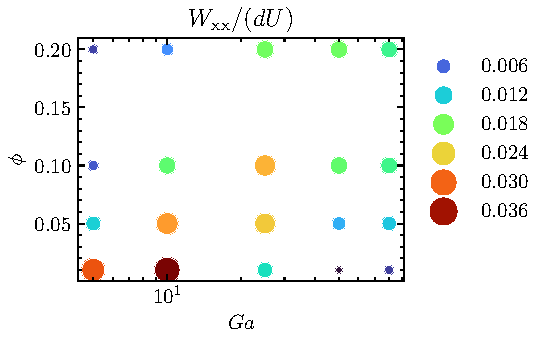
\includegraphics[height=5.5cm]{image/HOMOGENEOUS_NEW/PA/phase_Wxx_l_1.pdf}};
        \node (img) at (11,0) {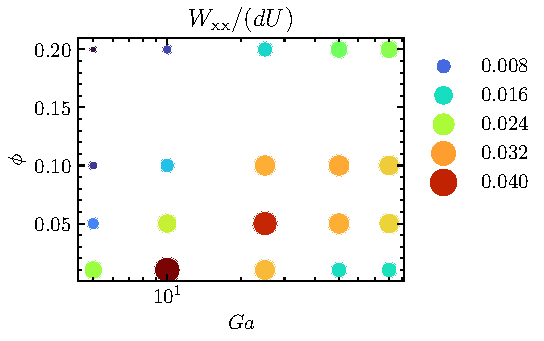
\includegraphics[height=5.5cm]{image/HOMOGENEOUS_NEW/PA/phase_Wxx_l_10.pdf}};
    \end{tikzpicture}
    \caption{Phase diagram of the horizontal components of the dimensionless correlation tensor $W_{xx}/(Ud)$. 
        (left) Iso-viscous emulsion $\lambda = 1$.
        (right) Viscous droplets $\lambda = 10$ }
    \label{fig:phase}
\end{figure}
Is the relative velocity fields $\textbf{w}_p^r$ the cause of the microstructure's shape as it is suggested by \ref{eq:dt_R}. 
Or does $\textbf{w}_p^r$ is the consequence of microstructure shape, as it could be through looking at the previous graphs ?
Indeed, on \ref{fig:Why_l_matter} (right), the clear asymmetry with respect to the horizontal plane can be explained as the consequence of cluster  in the flows. 
Although it is tedious question, we believe that both are true, even if physical parameters also impact $\textbf{w}_p^r$, which makes the microstructure case dependent.  
Nevertheless, this makes $\textbf{W}(\textbf{x},t)$ potentially a function of $\textbf{R}(\textbf{x},t)$.
Depending on its relationship with $\textbf{R}(\textbf{x},t)$ this might modify the relaxation time.  
Thus, a more efficient way to close \textbf{W} by an objective manner would be to study the dynamic of interactions. 
In this work we only provided a kinematics arguments to explain the microstructure shape. 
Of course to fully understand the physics one has to study the dynamic of interaction. 
It is in fact possible in our framework to include such dynamic variable by deriving an equation for \textbf{W} the same way we derived \ref{eq:dt_R} for \textbf{R}.
% In this case it is reasonable to believe that the closure terms for the dynamical equation might be computable theoretically in terms of the physical parameters $Ga$, $\phi$ and $\lambda$. 




% \subsection{Carrier phase velocity fields}

In the previous section we explained the microstructure formation with kinematic arguments.
Although we indeed provided an explanation the question that arise now id :
Why does the relative velocity behave as such.
The answer might be obtained based on dynamical arguments as it is done often, in such a way we could explain the relative kinematic.
Nevertheless, the dynamical aspect of the interaction is out of the scope of this study and will be treated in a future work. 

Instead, we propose to study the particles averaged wakes to explain the possible difference in interaction between the iso-viscous and viscous droplets cases. 
Again we make use of the nearest particle averaged statistic to compute the carrier fluid phase velocity conditionally on the presence of a particle at \textbf{x}, it reads,
\begin{equation*}
    \textbf{u}^\text{nst}_f P_{nst}(\textbf{x},\textbf{r},t)= 
    \int \sum_{i}^{N_b} \delta(\textbf{x}-\textbf{x}_i(\FF,t))
    h_{i} 
    \textbf{u}_f^0(\textbf{x}+\textbf{r},t,\FF)
    d\mathscr{P} 
\end{equation*}
where $h_{i} = 1$ if the particle $i$ center of mass is the nearest point to the eularian coordinate \textbf{x}+\textbf{r}. 
This velocity fields can be reconstructed as well with our DNS. 
On \ref{fig:stream} we display the reconstructed velocity field $\textbf{u}^\text{nst}_f$ for (left) the iso-viscous case $\lambda =1$ and (right) the viscous droplets' case $\lambda = 10$, for different value of the volume fraction. 
\begin{figure}[h!]
    \centering
    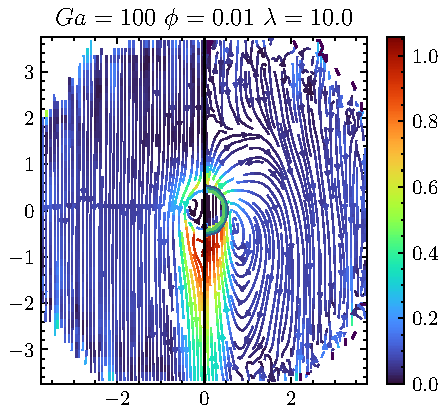
\includegraphics[height=0.4\textwidth]{image/HOMOGENEOUS_NEW/Stream/Stream_PHI_1_Ga_100_l_100}
    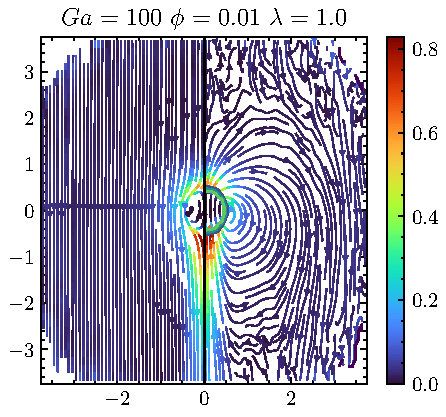
\includegraphics[height=0.4\textwidth]{image/HOMOGENEOUS_NEW/Stream/Stream_PHI_1_Ga_100_l_10}
    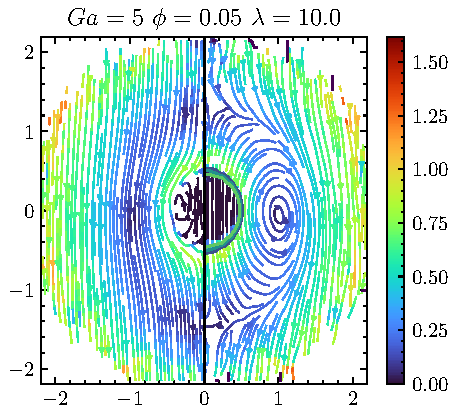
\includegraphics[height=0.4\textwidth]{image/HOMOGENEOUS_NEW/Stream/Stream_PHI_5_Ga_5_l_100}
    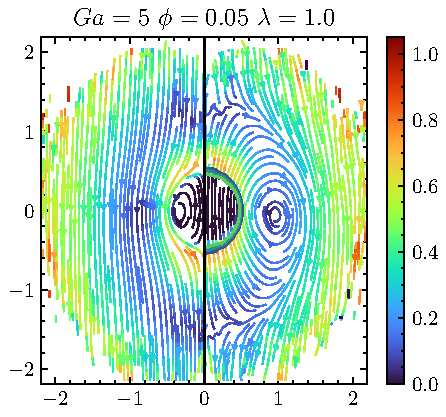
\includegraphics[height=0.4\textwidth]{image/HOMOGENEOUS_NEW/Stream/Stream_PHI_5_Ga_5_l_10}
    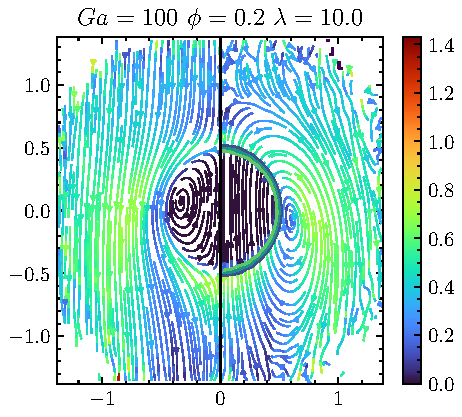
\includegraphics[height=0.4\textwidth]{image/HOMOGENEOUS_NEW/Stream/Stream_PHI_20_Ga_100_l_100}
    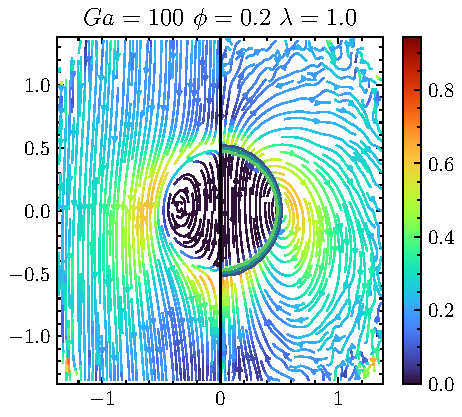
\includegraphics[height=0.4\textwidth]{image/HOMOGENEOUS_NEW/Stream/Stream_PHI_20_Ga_100_l_10}
    % 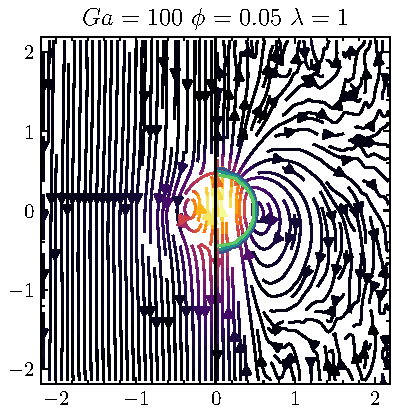
\includegraphics{image/HOMOGENEOUS_NEW/Stream/Stream_PHI_5_Ga_100_l_1.pdf}
    \caption{Nearest averaged carrier phase velocity fields. }
    \label{fig:stream}
\end{figure}
This velocity field is evaluated at $\textbf{x}+\textbf{r}$ conditioned on the presence of the nearest particle at $\textbf{x}$. 


\tb{compare with \citet{shajahan2023inertial} for explaination }

\section{Conclusion}
\section{Conclusion}

% \citet{einstein1905neue,taylor1932viscosity} demonstrated how the first moment of the hydrodynamic forces (Stresslet) applied on a particle immersed in pure linear flow induced an additional viscosity to the mixture. 
% Later~\citet{zhang1994ensemble,lhuillier1996contribution,jackson1997locally,zhang1997momentum} demonstrated that the second moment of forces were also contributing to the stresses inducing a non-newtonian behaviors, even in the Stokes and dilute limit.  

In this work we computed the moments of force on the surface of a test droplet in the situation of uniform relative motions between the droplet and the continuous phase. 
We considered low but finite Reynolds number $Re$. 
The averaged first moment of force is given by~\ref{eq:forces_reformulated2_avg}, scales as $O(\rho_f \phi u_r^2)$, hence contributing to the averaged Stress of the suspension on the same ground as  \citet{einstein1905neue} or \citep{taylor1932viscosity} correction to the viscosity of the mixture. 
In a lesser extend the inertial part of the second moment also contribute to the Rheology. 
This first point constitutes the main result of the paper. 

Others important conclusion reached through this work includes: a general reciprocal formula to derive the forces and moments on droplets, and the explicit appearing of the velocity variance term in the drag force term. 







\appendix

\section{Numerical validations}
\label{ap:validation}

The \texttt{Basilisk} code has been validated numerous time in previous numerical studies. 
Especially, we can cite the recent studies of \citet{innocenti2020direct} and \citet{hidman2023assessing} which both performed DNS of rising suspension of bubbles. 
Nevertheless, in this work we investigate specific statistical distribution,
and we make use of a multi-VoF method to avoid droplets coalescence, therefore a meticulous validation of the DNS is in order. 


\subsection*{Mesh independence and statistical convergence for random array of drops}

Even through aforementioned studies carried validation of the \texttt{Basilisk} code for rising droplets or bubbles, almost all of them considered isolated droplets or bubbles as the only validation case. 
As far as the author's knowledge, to this date no published study presented a mesh independence study for random array of droplets nor bubbles of this scale. 
Nevertheless, as particles interaction and higher \textit{Galileo} numbers may be more challenging to model, it is primordial to investigate the mesh independence of the exact same DNS that are carried in this work. 
In this objective we performed DNS of random array of $N_b=125$ droplets, with the following parameters,
\begin{align*}
    \lambda = 10,
    && \zeta = 1.11,
    && Bo = 1,
    && Ga = 100,
    && \phi = 0.1,
    && N_b =125,
\end{align*}
and the mesh definition is, $d/\Delta = 7.37, 14.74, 29.9 58.97$. 
We expect that the most challenging DNS simulated in this work is for the case, $\lambda = 10$ and $Ga = 100$, since it is in this range of parameters that we induce the most vorticity, which ultimately require good mesh definition. 
Additionally, in opposition to the ordered array case, this case includes droplets interaction, which ultimately induce more numerical complexities to tackles. 
Based on this remark we can assume that if this case is mesh independent, then all cases from \ref{tab:simulations} must be since this is the most challenging scenario.   

Now let's study the mesh influence on the statistics. 
It is clear from \ref{fig:apstat} (left) that both mesh definition produce nearly the same radial distribution, no notable difference is identified. 
In \ref{fig:apstat} (middle) we can observe the age distribution for both mesh definition. 
It is clear that refining the mesh induce a difference in the age distribution. 
As, a matter of fact it has a small impact on the mean age, $\tau_p = 6.96$ for the lower definition, and $\tau_p = 6.14$ for the finest grid.
This makes a $10\%$ error, but as mentioned above this is probably the highest error that we could encounter among all cases. 
\begin{figure}
    \centering
    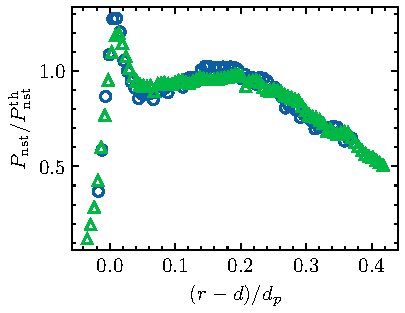
\includegraphics[height = 0.24\textwidth]{image/HOMOGENEOUS_NEW/VAL/Pr.pdf}
    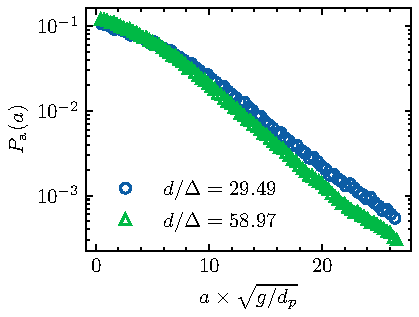
\includegraphics[height = 0.24\textwidth]{image/HOMOGENEOUS_NEW/VAL/Pa.pdf}
    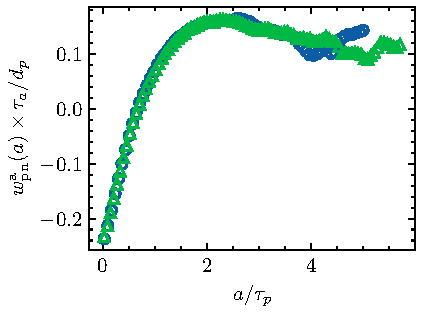
\includegraphics[height = 0.24\textwidth]{image/HOMOGENEOUS_NEW/VAL/w.pdf}
    \caption{
        Statistical averaged functions for two mesh definition. 
        (left) Radial normalized probability density function  $P_r(\textbf{x},|\textbf{r}|,t)/P_\text{th}$, in terms of the dimensionless radial position. 
        (middle) Probability density function of the age distribution $P_a(\textbf{x},t,a)$. 
        (right) Nearest averaged dimensionless approach velocity for both mesh definition, in terms of the dimensionless age. 
    }
    \label{fig:apstat}
\end{figure}
Even through an error is identified on the mean duration of interaction we still note that both nearest averaged dimensionless approach velocity on \ref{fig:apstat} (right) match perfectly. 
\begin{figure}[h!]
    \centering
    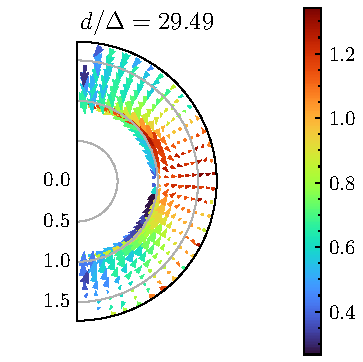
\includegraphics[height = 0.3\textwidth]{image/HOMOGENEOUS_NEW/VAL/U_rel_ndc_25.pdf}
    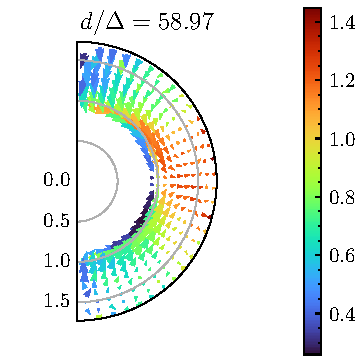
\includegraphics[height = 0.3\textwidth]{image/HOMOGENEOUS_NEW/VAL/U_rel_ndc_35.pdf}
    \caption{Quiver plots of the relative averaged velocity field $\textbf{w}^\text{r}(\textbf{x},\textbf{r},t)$ colored by the averaged dimensionless age $a^r(\textbf{x},\textbf{r},t)$, for $\phi = 0.05$ and $Ga = 100$. 
    (left) Low mesh definition.
    (right) High mesh definition. 
    }
    \label{fig:velap}
\end{figure}
Regarding, the 2D fields  $\textbf{w}^\text{r}(\textbf{x},\textbf{r},t)$ we can see that no notable difference can be identified, if it is not the slight difference in the value of the age scale. 


Overall, the one dimensional and two-dimensional conditioned statistics are almost independent of the mesh definition. 
By obtaining the same statistics with two independent DNS makes us confident on the fact that our numerical samples is large enough.
Indeed, if the samples were not sufficient we would have obtained two different distribution functions, thus we can be sure that the statistics have well converged. 
The slight difference in rising velocity (see \citet[Appendix A]{fintzi2024buoyancy}) and age distribution found for these Reynolds number must be acknowledged.
As mentioned at the beginning, this case is in fact very challenging as the volume fraction of droplets is consequent which induce numerous inertial interactions. 
Nevertheless, we can be sure that our final results is accurate at most with a $5\%$ error for this case, and probably less for the others cases. 
These, error testify for the very challenging  aspect of these simulations. 
Overall, we have great confidence in the statistical and physical representativity of our DNS results. 

\section{Additional information}
\label{ap:age} 

% \begin{table}[h!]
%     \caption{Performance of the different functions used in a tri-periodic simulations. In this case we set $N_b = 125$, $Ga = 25$, $\phi = 0.1$ $\lambda = 1$. }
%     \label{tab:performance}
%     \begin{tabular}{c|c|c|c|l}
%     calls  &  total  &   self &  total  & function\\\hline
%     11393554 &  5123.85  & 5123.85 &    27.5\% (25.1\% - 30.4\%) &  mpi\_boundary\_level():grid/multigrid-mpi.h:83\\
%     2723 &  2210.91 &  2207.58  &   11.8\% ( 6.0\% - 12.5\%)&   dump():output.h:1160\\
%    54442 &  3116.87 &  2012.52  &   10.8\% ( 9.6\% - 11.8\%)&   project():poisson.h:501\\
%  3449898 &  1344.44 &  1344.44  &    7.2\% ( 5.0\% - 12.0\%)&   mpi\_all\_reduce0():common.h:683\\
%   113949 &  2140.47 &  1314.60  &    7.0\% ( 6.5\% -  7.5\%)&   heights():heights.h:281\\
%    27221 &  2694.78 &  1197.03  &    6.4\% ( 5.8\% -  7.0\%)&   vof\_0():vof.h:365\\
%    27221 &  1974.21 &  1191.03  &    6.4\% ( 5.9\% -  6.9\%)&   viscosity():viscosity.h:173\\
%    27221 &  2441.96 &  924.93   &   5.0\% ( 4.4\% -  5.4\%) &  advection\_term():navier-stokes/centered.h:323\\
%    27221 &  1853.70 &  733.94   &   3.9\% ( 3.9\% -  4.0\%) &  no\_coalescence():no-coalescence.h:419\\
%     2723 &  3006.33 &  571.93   &   3.1\% ( 2.4\% -  3.4\%) &  track\_bub():RS.c:124\\
%   341847 &  564.43  & 344.91    &  1.8\% ( 1.6\% -  2.2\%)  & reconstruction():fractions.h:476\\
%   113949 &  2988.98 &  317.86   &   1.7\% ( 1.4\% -  2.2\%) &  curvature():curvature.h:621\\
%    78825 &  1158.49 &  294.73   &   1.6\% ( 1.3\% -  1.7\%) &  tag():tag.h:268\\
%    27221 &  336.74  & 203.09    &  1.1\% ( 1.0\% -  1.2\%)  & acceleration\_0():iforce.h:133\\
%    27221 &  2246.89 &  180.53   &   1.0\% ( 0.8\% -  1.1\%) &  projection():navier-stokes/centered.h:430\\
%    27221 &  2085.36 &  111.14   &   0.6\% ( 0.5\% -  0.7\%) &  viscous\_term():navier-stokes/centered.h:362\\
%    27221 &  137.78  & 108.82    &  0.6\% ( 0.5\% -  0.7\%)  & acceleration\_2():RS.c:166\\
%    27222 &  108.68  & 108.64    &  0.6\% ( 0.4\% -  0.6\%)  & properties\_0():two-phase-generic.h:101\\
%    27221 &  174.57  & 102.50    &  0.5\% ( 0.5\% -  0.6\%)  & acceleration():navier-stokes/centered.h:386\\
%    81548 &   83.75  &  83.71    &  0.4\% ( 0.4\% -  0.7\%)  & z\_indexing():grid/multigrid-mpi.h:145\\
%      118 &   59.37  &  59.37    &  0.3\% ( 0.2\% -  0.7\%)  & compose\_image():view.h:409\\
%    27221 &   66.24  &  34.89    &  0.2\% ( 0.2\% -  0.2\%)  & tracer\_advection\_1():no-coalescence.h:446\\
%       59 &  130.73  &  28.79    &  0.2\% ( 0.1\% -  0.2\%)  & movies():RS.c:244\\
%    27222 &  360.96  &  24.44    &  0.1\% ( 0.1\% -  0.2\%)  & stability\_1():tension.h:64\\
%    27222 &   25.28  &  20.61    &  0.1\% ( 0.1\% -  0.1\%)  & stability():navier-stokes/centered.h:226\\
% 44143779 &  3190.44 &    5.87   &   0.0\% ( 0.0\% -  0.0\%) &  boundary\_internal():grid/cartesian-common.h:45\\
% 42200829 &   27.27  &   3.67    &  0.0\% ( 0.0\% -  0.0\%)  & interpolate():grid/cartesian-common.h:815\\
%      550 &    2.34  &   2.34    &  0.0\% ( 0.0\% -  0.0\%)  & draw\_vof():draw.h:1052\\
%    67429 &   37.19  &   1.13    &  0.0\% ( 0.0\% -  0.0\%)  & reduce\_bubbles():no-coalescence.h:158\\
% \end{tabular}
% \end{table}

\begin{table}  
\begin{tabular}{c|c|c|c|l}
  calls  &  total  &   self  & \% total  & function \\ \hline
  10636901 &  4861.39 &  4861.39  &   31.8\% (28.4\% - 36.7\%) &   mpi\_boundary\_level():grid/multigrid-mpi.h:83\\
     53604 &  3097.64 &  1988.97  &   13.0\% (10.8\% - 14.7\%) &   project():poisson.h:501\\
     26802 &  2022.99 &  1236.57  &    8.1\% ( 7.3\% -  8.8\%) &   viscosity():viscosity.h:173\\
    107208 &  1984.59 &  1223.33  &    8.0\% ( 6.9\% -  8.9\%) &   heights():heights.h:281\\
     26802 &  2499.81 &  1099.66  &    7.2\% ( 6.1\% -  7.9\%) &   vof\_0():vof.h:365\\
   3155070 &  983.66  & 983.66    &  6.4\% ( 3.9\% -  9.1\%)   & mpi\_all\_reduce0():common.h:683\\
     26802 &  2372.23 &  896.09   &   5.9\% ( 5.1\% -  6.5\%)  &  advection\_term():navier-stokes/centered.h:323\\
     26802 &  1583.59 &  645.89   &   4.2\% ( 4.1\% -  4.3\%)  &  no\_coalescence():./no-coalescence.h:419\\
      2681 &  584.39  & 372.15    &  2.4\% ( 2.4\% -  2.5\%)   & track\_bub():RS.c:124\\
    321624 &  546.74  & 340.36    &  2.2\% ( 1.8\% -  2.6\%)   & reconstruction():fractions.h:476\\
    107208 &  2777.30 &  303.23   &   2.0\% ( 1.6\% -  2.4\%)  &  curvature():curvature.h:621\\
     69275 &  992.44  & 254.14    &  1.7\% ( 1.4\% -  1.8\%)   & tag():tag.h:268\\
     26802 &  328.67  & 202.85    &  1.3\% ( 1.1\% -  1.5\%)   & acceleration\_0():iforce.h:133\\
     26802 &  2257.27 &  178.19   &   1.2\% ( 0.8\% -  1.3\%)  &  projection():navier-stokes/centered.h:430\\
     26802 &  2142.30 &  119.30   &   0.8\% ( 0.5\% -  0.9\%)  &  viscous\_term():navier-stokes/centered.h:362\\
     26802 &  145.95  & 116.09    &  0.8\% ( 0.5\% -  0.9\%)   & acceleration\_2():RS.c:166\\
     26803 &  111.60  & 111.57    &  0.7\% ( 0.5\% -  0.8\%)   & properties\_0():two-phase-generic.h:101\\
     26802 &  172.09  & 100.18    &  0.7\% ( 0.5\% -  0.8\%)   & acceleration():navier-stokes/centered.h:386\\
     69275 &   68.91  &  68.88    &  0.5\% ( 0.4\% -  0.5\%)   & z\_indexing():grid/multigrid-mpi.h:145\\
       118 &   59.59  &  59.59    &  0.4\% ( 0.2\% -  0.8\%)   & compose\_image():view.h:409\\
     26802 &   64.69  &  34.48    &  0.2\% ( 0.2\% -  0.3\%)   & tracer\_advection\_1():./no-coalescence.h:446\\
        59 &  129.57  &  28.81    &  0.2\% ( 0.1\% -  0.2\%)   & movies():RS.c:244\\
     26803 &   92.48  &  27.24    &  0.2\% ( 0.1\% -  0.2\%)   & stability\_1():tension.h:64\\
     26803 &   24.42  &  21.33    &  0.1\% ( 0.1\% -  0.1\%)   & stability():navier-stokes/centered.h:226\\
  43894361 &  3001.24 &    5.50   &   0.0\% ( 0.0\% -  0.0\%)  &  boundary\_internal():grid/cartesian-common.h:450\\
  42061052 &   25.50  &   3.61    &  0.0\% ( 0.0\% -  0.0\%)   & interpolate():grid/cartesian-common.h:815\\
       472 &    2.31  &   2.31    &  0.0\% ( 0.0\% -  0.0\%)   & draw\_vof():draw.h:1052\\
     58554 &   25.92  &   0.87    &  0.0\% ( 0.0\% -  0.0\%)   & reduce\_bubbles():./no-coalescence.h:158\\
         1 &  15287.89&     0.73  &    0.0\% ( 0.0\% -  0.0\%) &   run():run.h:37\\
         1 &    0.28  &   0.28    &  0.0\% ( 0.0\% -  0.0\%)   & init\_0():RS.c:149\\
     26802 &  2777.57 &    0.27   &   0.0\% ( 0.0\% -  0.0\%)  &  acceleration\_1():tension.h:94\\
       236 &   38.81  &   0.21    &  0.0\% ( 0.0\% -  0.0\%)   & squares():draw.h:1375\\
    %    118 &   59.64  &   0.05    &  0.0\% ( 0.0\% -  0.1\%)   & save():view.h:529\\
    %  63404 &    0.06  &   0.03    &  0.0\% ( 0.0\% -  0.0\%)   & interpolate():grid/cartesian-common.h:816\\
    %      1 &    0.02  &   0.02    &  0.0\% ( 0.0\% -  0.0\%)   & defaults\_3():iforce.h:38\\
    %      1 &    0.01  &   0.01    &  0.0\% ( 0.0\% -  0.0\%)   & defaults\_2():two-phase-generic.h:26\\
    %  26802 &  1583.60 &    0.01   &   0.0\% ( 0.0\% -  0.0\%)  &  vof\_1():./no-coalescence.h:430\\
    %  26802 &    0.01  &   0.01    &  0.0\% ( 0.0\% -  0.0\%)   & set\_dtmax():navier-stokes/centered.h:222\\
    %  26803 &    0.00  &   0.00    &  0.0\% ( 0.0\% -  0.0\%)   & stability\_0():vof.h:143\\
    %      1 &    0.25  &   0.00    &  0.0\% ( 0.0\% -  0.0\%)   & init():navier-stokes/centered.h:213\\
    %      1 &    0.00  &   0.00    &  0.0\% ( 0.0\% -  0.0\%)   & defaults\_0():navier-stokes/centered.h:181\\
    %      1 &    0.00  &   0.00    &  0.0\% ( 0.0\% -  0.0\%)   & restore():output.h:1169\\
    %      1 &    0.00  &   0.00    &  0.0\% ( 0.0\% -  0.0\%)   & cleanup():run.h:52\\
    %      1 &    0.00  &   0.00    &  0.0\% ( 0.0\% -  0.0\%)   & defaults():run.h:44\\
    %      1 &    0.00  &   0.00    &  0.0\% ( 0.0\% -  0.0\%)   & defaults\_4():./no-coalescence.h:483\\
    %      1 &    0.00  &   0.00    &  0.0\% ( 0.0\% -  0.0\%)   & defaults\_1():vof.h:134\\
    %      1 &    0.00  &   0.00    &  0.0\% ( 0.0\% -  0.0\%)   & cleanup\_0():./no-coalescence.h:458\\
    %      1 &    0.00  &   0.00    &  0.0\% ( 0.0\% -  0.0\%)   & default\_display():navier-stokes/centered.h:188\\
    %      1 &    0.00  &   0.00    &  0.0\% ( 0.0\% -  0.0\%)   & stop():RS.c:272\\
\end{tabular}
\caption{Output of the basilisk compiler tool that measures algorithm performance all along the simulation.}
\end{table}



In this appendix we provide additional graph to support the argumentation made in the main text. 
Additional Radial distribution functions, 
\begin{figure}[h!]
    \centering
    % 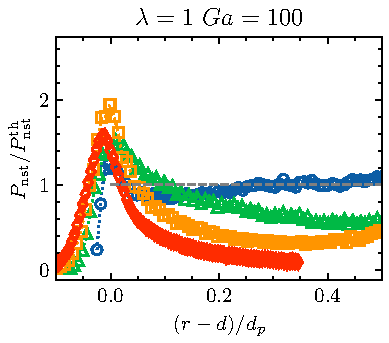
\includegraphics[height=0.3\textwidth]{image/HOMOGENEOUS_NEW/Dist/Pr_l_1_Ga_100.pdf}
    % 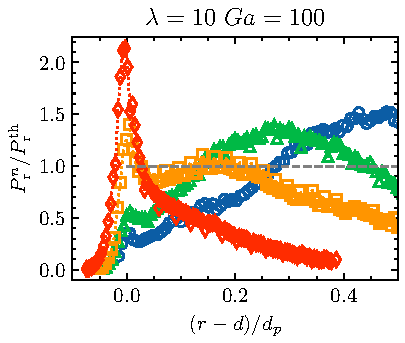
\includegraphics[height=0.3\textwidth]{image/HOMOGENEOUS_NEW/Dist/Pr_l_10_Ga_100.pdf}
    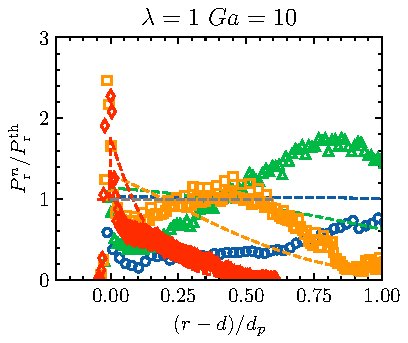
\includegraphics[height=0.3\textwidth]{image/HOMOGENEOUS_NEW/Dist/Pr_l_1_Ga_10.pdf}
    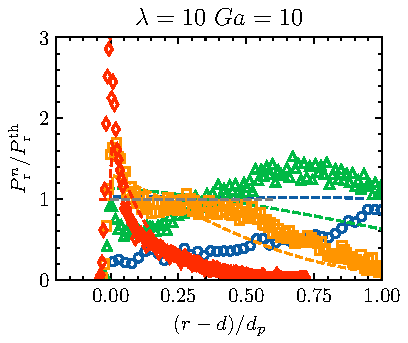
\includegraphics[height=0.3\textwidth]{image/HOMOGENEOUS_NEW/Dist/Pr_l_10_Ga_10.pdf}
    \caption{Radial probability density function $P_\text{nst}^n(\textbf{x},t,r)$ divided by the theoretical distribution $P_\text{nst}^{th}$ \ref{eq:Pnst_dilute}, in terms of the dimensionless distance $(r-d)/d_p$ where, $d_p = n_p^{-1/3}$, for  $Ga = 10$.
    (left)  $\lambda = 1$.
    (right) $\lambda = 10$.
    ($\pmb\bigcirc$) $\phi = 0.01$; ($\pmb\triangle$) $ \phi = 0.05$; ($\pmb\square$) $\phi = 0.1$ ($\pmb\lozenge$) $\phi = 0.2$.
    (dashed lines) Theoretical prediction : $P_\text{nst}^n/P_\text{nst}^\text{th} = 1$. 
    For $r<d$ we arbitrarily set $P_\text{nst}^\text{th} = 1$ so that the distribution can be visualized.
    }
    \label{fig:Pr_low}
\end{figure}
The drift velocity used in \ref{fig:age_picture} is given \ref{fig:Reall}.
\begin{figure}[h!]
    \centering
    \includegraphics[height = 0.3\textwidth]{image/HOMOGENEOUS_NEW/CA/Re_l_1.pdf}
    \includegraphics[height = 0.3\textwidth]{image/HOMOGENEOUS_NEW/CA/Re_l_10.pdf}
    \caption{
        Averaged Reynolds number based on the averaged drift velocity, $Re = \rho_fU d /\mu_f$, with $U = |\textbf{u}_p - \textbf{u}_f|$.
        $\textbf{u}_p$ and $\textbf{u}_f$ are the particle and fluid phase volume and time averaged velocity.
    }
    \label{fig:Reall}
\end{figure}
We provide additional age distribution for low \textit{Galileo} number to support the argumentation in the body of the text. 
\begin{figure}[h!]
    \centering
    \includegraphics[height = 0.3\textwidth]{image/HOMOGENEOUS_NEW/Dist/Pa_l_1_Ga_10.pdf}
    \includegraphics[height = 0.3\textwidth]{image/HOMOGENEOUS_NEW/Dist/Pa_l_10_Ga_10.pdf}
    \caption{(left) Age distribution at $\lambda = 10$ and $Ga = 10$ for : (solid line) $\phi = 0.2$; (dash dotted line) $\phi = 0.1$; (dashed line) $\phi =0.05$; (dotted line) $\phi = 0.01$. 
    (right) Mean dimensionless age in terms of the volume fraction $\phi$ for : 
    ($\pmb\bigcirc$) $Ga=1$; ($\pmb\triangle$) $ Ga = 10$; ($\pmb\square$) $Ga = 50$ ($\pmb\lozenge$) $Ga =100$.
    The age and $\tau_a$ are made dimensionless with $U/d$ where $U$ is the drift-velocity between the dispersed and continuous phase.  }
    \label{fig:age_picture_low_ga}
\end{figure}

\bibliography{Bib/bib_bulles.bib}

\end{document}

